\documentclass[]{book}
\usepackage{lmodern}
\usepackage{amssymb,amsmath}
\usepackage{ifxetex,ifluatex}
\usepackage{fixltx2e} % provides \textsubscript
\ifnum 0\ifxetex 1\fi\ifluatex 1\fi=0 % if pdftex
  \usepackage[T1]{fontenc}
  \usepackage[utf8]{inputenc}
\else % if luatex or xelatex
  \ifxetex
    \usepackage{mathspec}
  \else
    \usepackage{fontspec}
  \fi
  \defaultfontfeatures{Ligatures=TeX,Scale=MatchLowercase}
\fi
% use upquote if available, for straight quotes in verbatim environments
\IfFileExists{upquote.sty}{\usepackage{upquote}}{}
% use microtype if available
\IfFileExists{microtype.sty}{%
\usepackage{microtype}
\UseMicrotypeSet[protrusion]{basicmath} % disable protrusion for tt fonts
}{}
\usepackage[margin=1in]{geometry}
\usepackage{hyperref}
\hypersetup{unicode=true,
            pdftitle={Research methods for Psychology},
            pdfauthor={Matthew Crump},
            pdfborder={0 0 0},
            breaklinks=true}
\urlstyle{same}  % don't use monospace font for urls
\usepackage{natbib}
\bibliographystyle{apalike}
\usepackage{longtable,booktabs}
\usepackage{graphicx,grffile}
\makeatletter
\def\maxwidth{\ifdim\Gin@nat@width>\linewidth\linewidth\else\Gin@nat@width\fi}
\def\maxheight{\ifdim\Gin@nat@height>\textheight\textheight\else\Gin@nat@height\fi}
\makeatother
% Scale images if necessary, so that they will not overflow the page
% margins by default, and it is still possible to overwrite the defaults
% using explicit options in \includegraphics[width, height, ...]{}
\setkeys{Gin}{width=\maxwidth,height=\maxheight,keepaspectratio}
\IfFileExists{parskip.sty}{%
\usepackage{parskip}
}{% else
\setlength{\parindent}{0pt}
\setlength{\parskip}{6pt plus 2pt minus 1pt}
}
\setlength{\emergencystretch}{3em}  % prevent overfull lines
\providecommand{\tightlist}{%
  \setlength{\itemsep}{0pt}\setlength{\parskip}{0pt}}
\setcounter{secnumdepth}{5}
% Redefines (sub)paragraphs to behave more like sections
\ifx\paragraph\undefined\else
\let\oldparagraph\paragraph
\renewcommand{\paragraph}[1]{\oldparagraph{#1}\mbox{}}
\fi
\ifx\subparagraph\undefined\else
\let\oldsubparagraph\subparagraph
\renewcommand{\subparagraph}[1]{\oldsubparagraph{#1}\mbox{}}
\fi

%%% Use protect on footnotes to avoid problems with footnotes in titles
\let\rmarkdownfootnote\footnote%
\def\footnote{\protect\rmarkdownfootnote}

%%% Change title format to be more compact
\usepackage{titling}

% Create subtitle command for use in maketitle
\newcommand{\subtitle}[1]{
  \posttitle{
    \begin{center}\large#1\end{center}
    }
}

\setlength{\droptitle}{-2em}
  \title{Research methods for Psychology}
  \pretitle{\vspace{\droptitle}\centering\huge}
  \posttitle{\par}
  \author{Matthew Crump}
  \preauthor{\centering\large\emph}
  \postauthor{\par}
  \predate{\centering\large\emph}
  \postdate{\par}
  \date{2017-08-07}

\usepackage{booktabs}
\usepackage{amsthm}
\makeatletter
\def\thm@space@setup{%
  \thm@preskip=8pt plus 2pt minus 4pt
  \thm@postskip=\thm@preskip
}
\makeatother

\usepackage{amsthm}
\newtheorem{theorem}{Theorem}[chapter]
\newtheorem{lemma}{Lemma}[chapter]
\theoremstyle{definition}
\newtheorem{definition}{Definition}[chapter]
\newtheorem{corollary}{Corollary}[chapter]
\newtheorem{proposition}{Proposition}[chapter]
\theoremstyle{definition}
\newtheorem{example}{Example}[chapter]
\theoremstyle{remark}
\newtheorem*{remark}{Remark}
\begin{document}
\maketitle

{
\setcounter{tocdepth}{1}
\tableofcontents
}
\chapter{Psychological Science}\label{psychological-science}

Many people believe that women tend to talk more than men---with some
even suggesting that this difference has a biological basis. One widely
cited estimate is that women speak 20,000 words per day on average and
men speak only 7,000. This claim seems plausible, but is it true? A
group of psychologists led by Matthias Mehl decided to find out. They
checked to see if anyone had actually tried to count the daily number of
words spoken by women and men. No one had. So these researchers
conducted a study in which female and male college students (369 in all)
wore audio recorders while they went about their lives. The result? The
women spoke an average of 16,215 words per day and the men spoke an
average of 15,669---an extremely small difference that could easily be
explained by chance. In an article in the journal Science, these
researchers summed up their findings as follows: ``We therefore
conclude, on the basis of available empirical evidence, that the
widespread and highly publicized stereotype about female talkativeness
is unfounded'' (Mehl, Vazire, Ramirez-Esparza, Slatcher, \& Pennebaker,
2007, p.~82).

Science is a process for asking and answering questions about the world
around. It is a powerful tool for changing our own minds about how we
think the world works. For example, perhaps you too believed the
stereotype that women are more talkative than men. If so, science has
given you the opportunity to change your mind. The evidence collected so
far shows that there are no virtually no differences in the number of
words that women and men speak per day. If you choose to think like a
scientist, then you ought to change your belief and strongly consider
the possibility that the stereotype simply is not true. You might also
read the published journal article from the research described above to
critically evaluate how the research was conducted, and take a closer
look at the patterns in the data. After all, if you want to update your
beliefs on the basis of evidence, then you ought to make sure you can
trust the evidence.

This course is an introduction to the process of using the scientific
process to ask and answer questions relevant to psychologists. We will
talk about how to critically evaluate scientific findings so that we can
learn from the existing scientific literature. And, we will talk about
how to collect data to ask questions, and how to analyze data to answer
questions, so that we can contribute knowledge to the literature.

\section{Understanding Science}\label{understanding-science}

Psychology is usually defined as the scientific study of human behavior
and mental processes, and this example illustrates the features that
make it scientific. In this chapter, we look closely at these features,
introduce a model of scientific research in psychology, and address
several basic questions that students often have about it. Who conducts
scientific research in psychology? Why? Does scientific psychology tell
us anything that common sense does not? Why should I bother to learn the
scientific approach---especially if I want to be a clinical psychologist
and not a researcher? These are extremely good questions, and answering
them now will provide a solid foundation for learning the rest of the
material in your course.

\subsection{What Is Science?}\label{what-is-science}

Some people are surprised to learn that psychology is a science. They
generally agree that astronomy, biology, and chemistry are sciences but
wonder what psychology has in common with these other fields. Before
answering this question, however, it is worth reflecting on what
astronomy, biology, and chemistry have in common with each other. It is
clearly not their subject matter. Astronomers study celestial bodies,
biologists study living organisms, and chemists study matter and its
properties. It is also not the equipment and techniques that they use.
Few biologists would know what to do with a radio telescope, for
example, and few chemists would know how to track a moose population in
the wild. For these and other reasons, philosophers and scientists who
have thought deeply about this question have concluded that what the
sciences have in common is a general approach to understanding the
natural world. Psychology is a science because it takes this same
general approach to understanding one aspect of the natural world: human
behavior.

\subsection{Features of Science}\label{features-of-science}

The general scientific approach has three fundamental features
(Stanovich, 2010). The first is systematic empiricism. Empiricism refers
to learning based on observation, and scientists learn about the natural
world systematically, by carefully planning, making, recording, and
analyzing observations of it. As we will see, logical reasoning and even
creativity play important roles in science too, but scientists are
unique in their insistence on checking their ideas about the way the
world is against their systematic observations. Notice, for example,
that Mehl and his colleagues did not trust other people's stereotypes or
even their own informal observations. Instead, they systematically
recorded, counted, and compared the number of words spoken by a large
sample of women and men. Furthermore, when their systematic observations
turned out to conflict with people's stereotypes, they trusted their
systematic observations.

The second feature of the scientific approach---which follows in a
straightforward way from the first---is that it is concerned with
empirical questions. Empirical questions are questions that can be
answered by observations. These are questions about the way the world
actually is and, therefore, can be answered by systematically observing
it. The question of whether women talk more than men is empirical in
this way. Either women really do talk more than men or they do not, and
this can be determined by systematically observing how much women and
men actually talk. Having said this, there are many interesting and
important questions that are not empirically testable and that science
is not in a position to answer. Among these are questions about
values---whether things are good or bad, just or unjust, or beautiful or
ugly, and how the world ought to be. So, although the question of
whether a stereotype is accurate or inaccurate is an empirically
testable one that science can answer, the question---or, rather, the
value judgment---of whether it is wrong for people to hold inaccurate
stereotypes is not. Similarly, the question of whether criminal behavior
has a genetic basis is an empirical question, but the question of what
actions ought to be considered illegal is not. It is especially
important for researchers in psychology to be mindful of this
distinction.

The third feature of science is that it creates public knowledge. After
asking their empirical questions, making their systematic observations,
and drawing their conclusions, scientists publish their work. This
usually means writing an article for publication in a professional
journal, where they put their research question in the context of
previous research, describe in detail the methods they used to answer
their question, and clearly present their results and conclusions.
Increasingly, scientists are opting to publish their work in open access
journals so the articles are freely available to all -- scientists and
nonscientists alike. This important choice allows publicly-funded
research to create knowledge that is truly public.

Publication is an essential feature of science for two reasons. One is
that science is a social process---a large-scale collaboration among
many researchers distributed across both time and space. Our current
scientific knowledge of most topics is based on many different studies
conducted by many different researchers who have shared their work
publicly over many years. The second is that publication allows science
to be self-correcting. Individual scientists understand that, despite
their best efforts, their methods can be flawed and their conclusions
incorrect. Publication allows others in the scientific community to
detect and correct these errors so that, over time, scientific knowledge
increasingly reflects the way the world actually is.

A good example of the self-correcting nature of science is the ``Many
Labs Replication Project'' -- a large and coordinated effort by
prominent psychological scientists around the world to attempt to
replicate findings from 13 classic and contemporary studies (Klein et
al., 2013). One of the findings selected by these researchers for
replication was the fascinating effect, first reported by Simone Schnall
and her colleagues at the University of Plymouth, that washing one's
hands leads people to view moral transgressions---ranging from keeping
money inside a found wallet, to using a kitten for sexual arousal---as
less wrong (Schnall, Benton, \& Harvey, 2008). If reliable, this effect
might help explain why so many religious traditions associate physical
cleanliness with moral purity. However, despite using the same materials
and nearly identical procedures with a much larger sample, the ``Many
Labs'' researchers were unable to replicate the original finding
(Johnson, Cheung, \& Donnellan, 2013)4, suggesting that the original
finding may have stemmed from the relatively small sample size (which
can lead to unreliable results) used in the original study. To be clear,
at this stage we are still unable to definitively conclude that the
handwashing effect does not exist; however, the effort that has gone
into testing its reliability certainly demonstrates the collaborative
and cautious nature of scientific progress.

\subsection{Science Versus
Pseudoscience}\label{science-versus-pseudoscience}

Pseudoscience refers to activities and beliefs that are claimed to be
scientific by their proponents---and may appear to be scientific at
first glance---but are not. Consider the theory of biorhythms (not to be
confused with sleep cycles or other biological cycles that do have a
scientific basis). The idea is that people's physical, intellectual, and
emotional abilities run in cycles that begin when they are born and
continue until they die. Allegedly, the physical cycle has a period of
23 days, the intellectual cycle a period of 33 days, and the emotional
cycle a period of 28 days. So, for example, if you had the option of
when to schedule an exam, you would want to schedule it for a time when
your intellectual cycle will be at a high point. The theory of
biorhythms has been around for more than 100 years, and you can find
numerous popular books and websites about biorhythms, often containing
impressive and scientific-sounding terms like sinusoidal wave and
bioelectricity. The problem with biorhythms, however, is that there is
simply no evidence for them, so there is no good reason to think they
exist (Hines, 1998).

A set of beliefs or activities can be said to be pseudoscientific if (a)
its adherents claim or imply that it is scientific, but (b) it lacks one
or more of the three features of science. For instance, it might lack
systematic empiricism. Either there is no relevant scientific research
or, as in the case of biorhythms, there is relevant scientific research
but it is ignored. It might also lack public knowledge. People who
promote the beliefs or activities might claim to have conducted
scientific research but never publish that research in a way that allows
others to evaluate it.

A set of beliefs and activities might also be pseudoscientific because
it does not address empirical questions. The philosopher Karl Popper was
especially concerned with this idea (Popper, 2002). He argued more
specifically that any scientific claim must be expressed in such a way
that there are observations that would---if they were made---count as
evidence against the claim. In other words, scientific claims must be
\emph{falsifiable}. The claim that women talk more than men is
falsifiable because systematic observations could reveal either that
they do talk more than men or that they do not. As an example of an
unfalsifiable claim, consider that many people who believe in
extrasensory perception (ESP) and other psychic powers claim that such
powers can disappear when they are observed too closely. This makes it
so that no possible observation would count as evidence against ESP. If
a careful test of a self-proclaimed psychic showed that she predicted
the future at better-than-chance levels, this would be consistent with
the claim that she had psychic powers. But if she failed to predict the
future at better-than-chance levels, this would also be consistent with
the claim because her powers can supposedly disappear when they are
observed too closely.

Why should we concern ourselves with pseudoscience? There are at least
three reasons. One is that learning about pseudoscience helps bring the
fundamental features of science---and their importance---into sharper
focus. A second is that biorhythms, psychic powers, astrology, and many
other pseudoscientific beliefs are widely held and are promoted on the
Internet, on television, and in books and magazines. Far from being
harmless, the promotion of these beliefs often results in great personal
toll as, for example, believers in pseudoscience opt for ``treatments''
such as homeopathy for serious medical conditions instead of
empirically-supported treatments. Learning what makes them
pseudoscientific can help us to identify and evaluate such beliefs and
practices when we encounter them. A third reason is that many
pseudoscience's purport to explain some aspect of human behavior and
mental processes, including biorhythms, astrology, graphology
(handwriting analysis), and magnet therapy for pain control. It is
important for students of psychology to distinguish their own field
clearly from this ``pseudo psychology.''

\subsection{Key Takeaways}\label{key-takeaways}

\begin{itemize}
\item
  Science is a general way of understanding the natural world. Its three
  fundamental features are systematic empiricism, empirical questions,
  and public knowledge.
\item
  Psychology is a science because it takes the scientific approach to
  understanding human behavior.
\item
  Pseudoscience refers to beliefs and activities that are claimed to be
  scientific but lack one or more of the three features of science. It
  is important to distinguish the scientific approach to understanding
  human behavior from the many pseudoscientific approaches.
\end{itemize}

\subsection{Exercises}\label{exercises}

\begin{enumerate}
\def\labelenumi{\arabic{enumi}.}
\item
  Practice: List three empirical questions about human behavior. List
  three nonempirical questions about human behavior.
\item
  Discussion: Consider the following psychological claim. ``People's
  choice of spouse is strongly influenced by their perception of their
  own parents. Some choose a spouse who is similar in some way to one of
  their parents. Others choose a spouse who is different from one of
  their parents.'' Is this claim falsifiable? Why or why not?
\item
  Discussion: People sometimes suggest that psychology cannot be a
  science because either (a) human behavior cannot be predicted with
  perfect accuracy or (b) much of its subject matter (e.g., thoughts and
  feelings) cannot be observed directly. Do you agree or disagree with
  each of these ideas? Why?
\item
  Watch the following video by PHD Comics for an overview of open access
  publishing and why it matters.
  \url{https://www.youtube.com/watch?v=L5rVH1KGBCY}
\end{enumerate}

\section{Scientific Research in
Psychology}\label{scientific-research-in-psychology}

\subsection{A Model of Scientific Research in
Psychology}\label{a-model-of-scientific-research-in-psychology}

\begin{figure}

{\centering 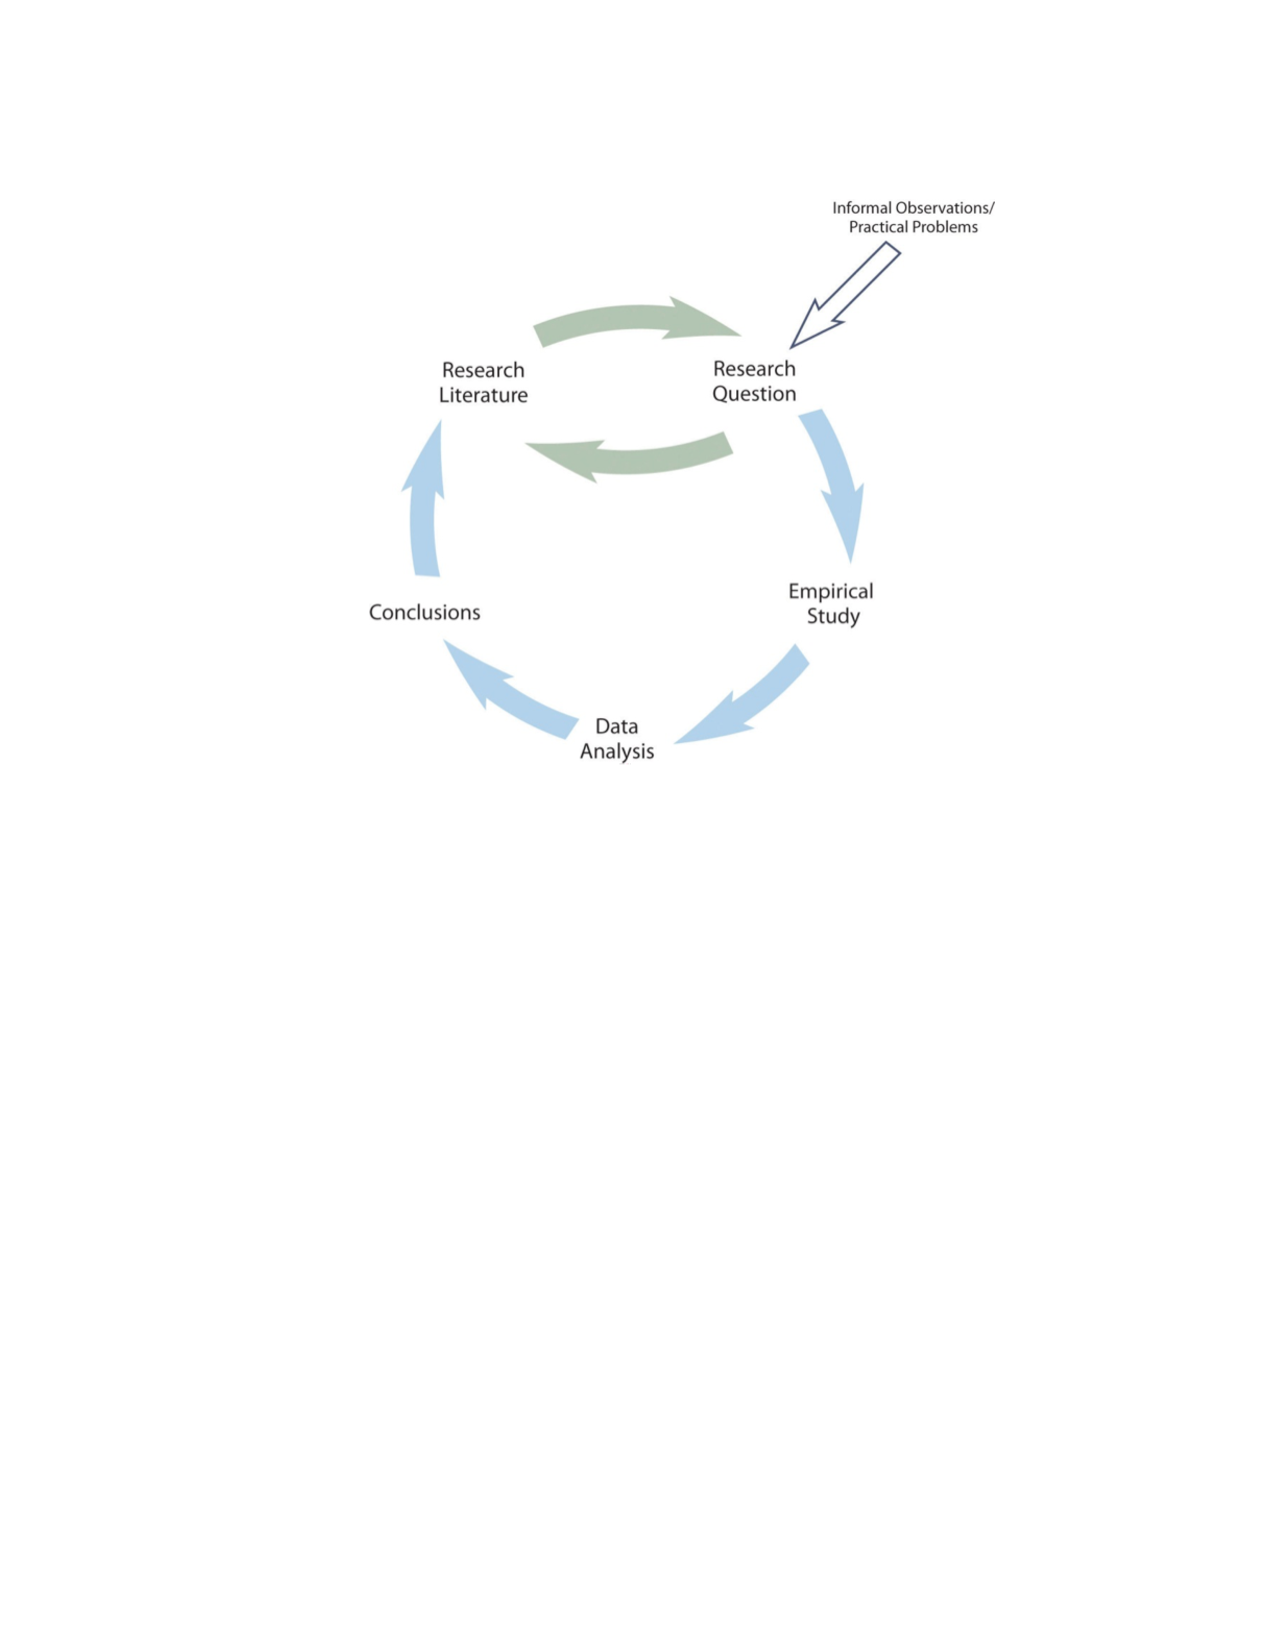
\includegraphics[width=0.5\linewidth]{figures/C1Figure1} 

}

\caption{This is a caption}\label{fig:Theresearchcycle}
\end{figure}

Figure \ref{fig:Theresearchcycle} presents a more specific model of
scientific research in psychology. The researcher (who more often than
not is really a small group of researchers) formulates a research
question, conducts a study designed to answer the question, analyzes the
resulting data, draws conclusions about the answer to the question, and
publishes the results so that they become part of the research
literature. Because the research literature is one of the primary
sources of new research questions, this process can be thought of as a
cycle. New research leads to new questions, which lead to new research,
and so on. Figure \ref{fig:Theresearchcycle} also indicates that
research questions can originate outside of this cycle either with
informal observations or with practical problems that need to be solved.
But even in these cases, the researcher would start by checking the
research literature to see if the question had already been answered and
to refine it based on what previous research had already found.

The research by Mehl and his colleagues is described nicely by this
model. Their question---whether women are more talkative than men---was
suggested to them both by people's stereotypes and by published claims
about the relative talkativeness of women and men. When they checked the
research literature, however, they found that this question had not been
adequately addressed in scientific studies. They then conducted a
careful empirical study, analyzed the results (finding very little
difference between women and men), and published their work so that it
became part of the research literature. The publication of their article
is not the end of the story, however, because their work suggests many
new questions (about the reliability of the result, about potential
cultural differences, etc.) that will likely be taken up by them and by
other researchers inspired by their work.

As another example, consider that as cell phones became more widespread
during the 1990s, people began to wonder whether, and to what extent,
cell phone use had a negative effect on driving. Many psychologists
decided to tackle this question scientifically (Collet, Guillot, \&
Petit, 2010). It was clear from previously published research that
engaging in a simple verbal task impairs performance on a perceptual or
motor task carried out at the same time, but no one had studied the
effect specifically of cell phone use on driving. Under carefully
controlled conditions, these researchers compared people's driving
performance while using a cell phone with their performance while not
using a cell phone, both in the lab and on the road. They found that
people's ability to detect road hazards, reaction time, and control of
the vehicle were all impaired by cell phone use. Each new study was
published and became part of the growing research literature on this
topic.

\subsection{Who Conducts Scientific Research in
Psychology?}\label{who-conducts-scientific-research-in-psychology}

Scientific research in psychology is generally conducted by people with
doctoral degrees (usually the doctor of philosophy, PhD) and master's
degrees in psychology and related fields, often supported by research
assistants with bachelor's degrees or other relevant training. Some of
them work for government agencies (e.g., the National Institute of
Health), national associations (e.g., the American Psychological
Association), nonprofit organizations (e.g., the Canadian Mental Health
Association), or in the private sector (e.g., in product development).
However, the majority of them are college and university faculty, who
often collaborate with their graduate and undergraduate students.
Although some researchers are trained and licensed as
clinicians---especially those who conduct research in clinical
psychology---the majority are not. Instead, they have expertise in one
or more of the many other subfields of psychology: behavioral
neuroscience, cognitive psychology, developmental psychology,
personality psychology, social psychology, and so on. Doctoral-level
researchers (post-doctoral fellows or research scientists) might be
employed to conduct research full-time or, like many college and
university faculty members, to conduct research in addition to teaching
classes and serving their institution and community in other ways.

Of course, people also conduct research in psychology because they enjoy
the intellectual and technical challenges involved and the satisfaction
of contributing to scientific knowledge of human behavior. You might
find that you enjoy the process too. If so, your college or university
might offer opportunities to get involved in ongoing research as either
a research assistant or a participant.

Of course, you might find that you do not enjoy the process of
conducting scientific research in psychology. But at least you will have
a better understanding of where scientific knowledge in psychology comes
from, an appreciation of its strengths and limitations, and an awareness
of how it can be applied to solve practical problems in psychology and
everyday life.

\subsection{The Broader Purposes of Scientific Research in
Psychology}\label{the-broader-purposes-of-scientific-research-in-psychology}

People have always been curious about the natural world, including
themselves and their behavior (in fact, this is probably why you are
studying psychology in the first place). Science grew out of this
natural curiosity and has become the best way to achieve detailed and
accurate knowledge. Keep in mind that most of the phenomena and theories
that fill psychology textbooks are the products of scientific research.
In a typical introductory psychology textbook, for example, one can
learn about specific cortical areas for language and perception,
principles of classical and operant conditioning, biases in reasoning
and judgment, and people's surprising tendency to obey those in
positions of authority. And scientific research continues because what
we know right now only scratches the surface of what we can know.

Scientific research is often classified as being either \emph{basic} or
\emph{applied}. Basic research in psychology is conducted primarily for
the sake of achieving a more detailed and accurate understanding of
human behavior, without necessarily trying to address any particular
practical problem. The research of Mehl and his colleagues falls into
this category. Applied research is conducted primarily to address some
practical problem. Research on the effects of cell phone use on driving,
for example, was prompted by safety concerns and has led to the
enactment of laws to limit this practice. Although the distinction
between basic and applied research is convenient, it is not always
clear-cut. For example, basic research on sex differences in
talkativeness could eventually have an effect on how marriage therapy is
practiced, and applied research on the effect of cell phone use on
driving could produce new insights into basic processes of perception,
attention, and action.

\subsection{Key Takeaways}\label{key-takeaways-1}

\begin{itemize}
\item
  Research in psychology can be described by a simple cyclical model. A
  research question based on the research literature leads to an
  empirical study, the results of which are published and become part of
  the research literature.
\item
  Scientific research in psychology is conducted mainly by people with
  doctoral degrees in psychology and related fields, most of whom are
  college and university faculty members. They do so for professional
  and for personal reasons, as well as to contribute to scientific
  knowledge about human behavior.
\item
  Basic research is conducted to learn about human behavior for its own
  sake, and applied research is conducted to solve some practical
  problem. Both are valuable, and the distinction between the two is not
  always clear-cut.
\end{itemize}

\subsection{Exercises}\label{exercises-1}

\begin{enumerate}
\def\labelenumi{\arabic{enumi}.}
\item
  Practice: Find a description of an empirical study in a professional
  journal or in one of the scientific psychology blogs. Then write a
  brief description of the research in terms of the cyclical model
  presented here. One or two sentences for each part of the cycle should
  suffice.
\item
  Practice: Based on your own experience or on things you have already
  learned about psychology, list three basic research questions and
  three applied research questions of interest to you.
\item
  Watch the following TED Ed video
  \href{https://youtu.be/\%20GUpd2HJHUt8}{https://youtu.be/
  GUpd2HJHUt8}, in which David H. Schwartz provides an introduction to
  two types of empirical studies along with some methods that scientists
  use to increase the reliability of their results.
\end{enumerate}

\section{Science and Common Sense}\label{science-and-common-sense}

\subsection{Can We Rely on Common
Sense?}\label{can-we-rely-on-common-sense}

Some people wonder whether the scientific approach to psychology is
necessary. Can we not reach the same conclusions based on common sense
or intuition? Certainly we all have intuitive beliefs about people's
behavior, thoughts, and feelings---and these beliefs are collectively
referred to as folk psychology. Although much of our folk psychology is
probably reasonably accurate, it is clear that much of it is not. For
example, most people believe that anger can be relieved by ``letting it
out''---perhaps by punching something or screaming loudly. Scientific
research, however, has shown that this approach tends to leave people
feeling more angry, not less (Bushman, 2002). Likewise, most people
believe that no one would confess to a crime that he or she had not
committed, unless perhaps that person was being physically tortured. But
again, extensive empirical research has shown that false confessions are
surprisingly common and occur for a variety of reasons (Kassin \&
Gudjonsson, 2004). There are many more examples where our own intuitions
about ourselves and others are incorrect.

\subsection{How Could We Be So Wrong?}\label{how-could-we-be-so-wrong}

How can so many of our intuitive beliefs about human behavior be so
wrong? Notice that this is an empirical question, and it just so happens
that psychologists have conducted scientific research on it and
identified many contributing factors (Gilovich, 1991). One is that
forming detailed and accurate beliefs requires powers of observation,
memory, and analysis to an extent that we do not naturally possess. It
would be nearly impossible to count the number of words spoken by the
women and men we happen to encounter, estimate the number of words they
spoke per day, average these numbers for both groups, and compare
them---all in our heads. This is why we tend to rely on mental shortcuts
(what psychologists refer to as heuristics) in forming and maintaining
our beliefs. For example, if a belief is widely shared---especially if
it is endorsed by ``experts''---and it makes intuitive sense, we tend to
assume it is true. This is compounded by the fact that we then tend to
focus on cases that confirm our intuitive beliefs and not on cases that
dis-confirm them. This is called \emph{confirmation bias}. For example,
once we begin to believe that women are more talkative than men, we tend
to notice and remember talkative women and silent men but ignore or
forget silent women and talkative men. We also hold incorrect beliefs in
part because it would be nice if they were true. For example, many
people believe that calorie-reducing diets are an effective long- term
treatment for obesity, yet a thorough review of the scientific evidence
has shown that they are not (Mann et al., 2007)5. People may continue to
believe in the effectiveness of dieting in part because it gives them
hope for losing weight if they are obese or makes them feel good about
their own ``self-control'' if they are not.

Scientists---especially psychologists---understand that they are just as
susceptible as anyone else to intuitive but incorrect beliefs. This is
why they cultivate an attitude of \emph{skepticism}. Being skeptical
does not mean being cynical or distrustful, nor does it mean questioning
every belief or claim one comes across (which would be impossible
anyway). Instead, it means pausing to consider alternatives and to
search for evidence---especially systematically collected empirical
evidence---when there is enough at stake to justify doing so. For
example, imagine that you read a magazine article claiming that giving
children a weekly allowance is a good way to help them develop financial
responsibility. This is an interesting and potentially important claim
(especially if you have children of your own). Taking an attitude of
skepticism, however, would mean pausing to ask whether it might be
instead that receiving an allowance merely teaches children to spend
money---perhaps even to be more materialistic. Taking an attitude of
skepticism would also mean asking what evidence supports the original
claim. Is the author a scientific researcher? Is any scientific evidence
cited? If the issue was important enough, it might also mean turning to
the research literature to see if anyone else had studied it. Then, you
could evaluate the existing evidence yourself to determine whether the
evidence supports the claim.

Because there is often not enough evidence to fully evaluate a belief or
claim, scientists also cultivate a tolerance for uncertainty. They
accept that there are many things that they simply do not know. For
example, it turns out that there is no scientific evidence that
receiving an allowance causes children to be more financially
responsible, nor is there any scientific evidence that it causes them to
be materialistic. Although this kind of uncertainty can be problematic
from a practical perspective---for example, making it difficult to
decide what to do when our children ask for an allowance---it is
exciting from a scientific perspective. If we do not know the answer to
an interesting and empirically testable question, science, and perhaps
even you as a researcher, may be able to provide the answer.

\subsection{Key Takeaways}\label{key-takeaways-2}

\begin{itemize}
\item
  People's intuitions about human behavior, also known as folk
  psychology, often turn out to be wrong. This is one primary reason
  that psychology relies on science rather than common sense.
\item
  Researchers in psychology cultivate certain critical-thinking
  attitudes. One is skepticism. They search for evidence and consider
  alternatives before accepting a claim about human behavior as true.
  Another is tolerance for uncertainty. They withhold judgment about
  whether a claim is true or not when there is insufficient evidence to
  decide.
\end{itemize}

\subsection{Exercises}\label{exercises-2}

\begin{enumerate}
\def\labelenumi{\arabic{enumi}.}
\item
  Practice: For each of the following intuitive beliefs about human
  behavior, list three reasons that it might be true and three reasons
  that it might not be true:

  \begin{itemize}
  \item
    You cannot truly love another person unless you love yourself.
  \item
    People who receive ``crisis counseling'' immediately after
    experiencing a traumatic event are better able to cope with that
    trauma in the long term.
  \item
    Studying is most effective when it is always done in the same
    location.
  \end{itemize}
\item
  Watch the following video, in which psychologist Scott Lilienfeld
  talks about confirmation bias, tunnel vision, and using evidence to
  evaluate the world around us
  \href{https://youtu.be/\%20Eut8jMfSA_k}{https://youtu.be/
  Eut8jMfSA\_k}
\end{enumerate}

\section{Science and Clinical
Practice}\label{science-and-clinical-practice}

Psychology is the scientific study of behavior and mental processes. But
it is also the application of scientific research to ``help people,
organizations, and communities function better'' (American Psychological
Association, 2011). By far the most common and widely known application
is the clinical practice of psychology---the diagnosis and treatment of
psychological disorders and related problems. Let us use the term
clinical practice broadly to refer to the activities of clinical and
counseling psychologists, school psychologists, marriage and family
therapists, licensed clinical social workers, and others who work with
people individually or in small groups to identify and help address
their psychological problems. It is important to consider the
relationship between scientific research and clinical practice because
many students are especially interested in clinical practice, perhaps
even as a career.

The main point is that psychological disorders and other behavioral
problems are part of the natural world. This means that questions about
their nature, causes, and consequences are empirically testable and
therefore subject to scientific study. As with other questions about
human behavior, we cannot rely on our intuition or common sense for
detailed and accurate answers. Consider, for example, that dozens of
popular books and thousands of websites claim that adult children of
alcoholics have a distinct personality profile, including low
self-esteem, feelings of powerlessness, and difficulties with intimacy.
Although this sounds plausible, scientific research has demonstrated
that adult children of alcoholics are no more likely to have these
problems than anybody else (Lilienfeld et al., 2010). Similarly,
questions about whether a particular psychotherapy is effective are
empirically testable questions that can be answered by scientific
research. If a new psychotherapy is an effective treatment for
depression, then systematic observation should reveal that depressed
people who receive this psychotherapy improve more than a similar group
of depressed people who do not receive this psychotherapy (or who
receive some alternative treatment). Treatments that have been shown to
work in this way are called \textbf{empirically supported treatments}.

Many in the clinical psychology community have argued that their field
has not paid enough attention to scientific research---for example, by
failing to use empirically supported treatments---and have suggested a
variety of changes in the way clinicians are trained and treatments are
evaluated and put into practice. Others believe that these claims are
exaggerated and the suggested changes are unnecessary (Norcross,
Beutler, \& Levant, 2005). On both sides of the debate, however, there
is agreement that a scientific approach to clinical psychology is
essential if the goal is to diagnose and treat psychological problems
based on detailed and accurate knowledge about those problems and the
most effective treatments for them. So not only is it important for
scientific research in clinical psychology to continue, but it is also
important for clinicians who never conduct a scientific study themselves
to be scientifically literate so that they can read and evaluate new
research and make treatment decisions based on the best available
evidence.

\subsection{Key Takeaways}\label{key-takeaways-3}

\begin{itemize}
\item
  The clinical practice of psychology---the diagnosis and treatment of
  psychological problems---is one important application of the
  scientific discipline of psychology.
\item
  Scientific research is relevant to clinical practice because it
  provides detailed and accurate knowledge about psychological problems
  and establishes whether treatments are effective.
\end{itemize}

\subsection{Exercises}\label{exercises-3}

\begin{enumerate}
\def\labelenumi{\arabic{enumi}.}
\item
  Discussion: Some clinicians argue that what they do is an ``art form''
  based on intuition and personal experience and therefore cannot be
  evaluated scientifically. Write a paragraph about how satisfied you
  would be with such a clinician and why from each of three
  perspectives:

  \begin{itemize}
  \item
    a potential client of the clinician
  \item
    a judge who must decide whether to allow the clinician to testify as
    an expert witness in a child abuse case
  \item
    an insurance company representative who must decide whether to
    reimburse the clinician for his or her services
  \end{itemize}
\item
  Practice: Create a short list of questions that a client could ask a
  clinician to determine whether he or she pays sufficient attention to
  scientific research.
\end{enumerate}

\section{Using Psychological Science to Inform Your
Worldview}\label{using-psychological-science-to-inform-your-worldview}

Psychology is a very broad scientific discipline that asks and answers
all sorts of questions about human and non-human animals. Psychological
science encompasses many levels of analysis spanning the building blocks
of biological systems, such as genes and cells, neurochemistry, neurons,
and networks of neurons; perceptual and cognitive abilities of
individuals such as learning, memory, attention, decision-making,
language, thought, intelligence, and consciousness, to complex aspects
of individuals such as development, personality, social behavior, and
many others. A typical introductory psychology has the difficult job of
presenting a bird's eye view of all of these major psychological domains
of inquiry. Although psychologists ask many different kinds of
questions, they all employ the scientific method as a tool to answer
questions. So, this course is an introduction to the scientific research
methods that are used in all areas of Psychology.

The primary focus of the course will be on experiments, which is the
most powerful empirical tool researchers have to determine the
underlying causes of the psychological phenomena that they measure.
Psychological research methods are not limited to experiments, and
non-experimental, or quasi-experimental approaches are often used with
great success to ask and answer questions. Some of these research
methods will be highlighted throughout the course.

\subsection{Why Should I Care About How Psychology Experiments
work?}\label{why-should-i-care-about-how-psychology-experiments-work}

Imagine for the moment a world without experiments that does not use the
scientific method. This world would still have people claiming to have
knowledge about how things work, and it would still have tools and
technologies that are claimed to solve particular problems. However,
without experiments to test whether the claims are true, all we are left
with is the untested claims that may be true or false. We would be left
in the dark. Inevitably, and not too different from our world today,
there would be large segments of the population who believe false claims
about how things work, and large segments of the population using
therapies, tools, or other technologies that simply do not work (even if
they believe they do).

The world we live in today discovered the scientific method and uses
experiments to test claims about how things work. Indeed, with the
enormous number of ways that we receive information through the media
today, it is difficult to avoid hearing about all sorts of new
scientific claims as well as totally unfounded claims that may not be
based in science. For example, we have probably all heard that eating
too much of something is good or bad for you, and increases or decreases
your risk for a health problem. These claims can even flip around so
that last year eating too much of X was bad, but this year eating too
little of X is bad. What's more, many of these claims are supposedly
scientific ones based on experiments. Should you believe these claims,
and should you change your own behavior because of them?

When we receive claims through the media we are getting second-hand
information, and based on this information alone it is difficult to
evaluate the claim and the evidence for the claim. One option is to find
expert reporters that you trust, and then believe everything they say.
The second option is to find the primary source, and then evaluate the
evidence yourself to determine whether you should believe the claim. The
ability to understand how experiments work gives you the tools you need
to critically evaluate claims about how things work.

\subsection{Evaluating Claims}\label{evaluating-claims}

It is an understatement to say that people believe all sorts of crazy
things. Note, this is a claim that I just made. Should you believe it?
What do you need to know to determine whether or not you should believe
this claim or any other claim? Scientific thinking requires that claims
are supported by evidence. Other forms of belief and thinking may not
require evidence to support claims.

For the moment I'll put on my scientific thinking hat because there
numerous ways that I can provide evidence for my claim the people
believe all sorts of crazy things. I am a person, and I know that I have
believed crazy things in the past. For example, when I was four I
believed that all children grow to be taller than their parents because
I visited a family who had many children of different ages, and the
oldest ones were all taller than their parents. I believed this claim
for many years until finding out at the age of 12 that all of the
children in that family were adopted (nevertheless, I am taller than
both my parents, but my brother is not, so much for my theory). The
internet is full of people claiming to believe things that I think are
completely crazy. For example, the flat earth society believes that the
earth is flat and shaped like a frisbee. Believers in the great
reptilian conspiracy maintain that many of our world leaders are lizard
people. The abundance of conspiracy theories provides a deep well of
evidence that people believe all sorts of crazy things. So, because I
can back up my claim with evidence, I will continue believing that
people believe all sorts of crazy things.

I could also take my science hat off, and then I can believe anything I
want. Indeed, this remarkable imagination ability may be one reason why
people believe so many crazy things without needing any evidence
whatsoever to back up their beliefs. I can believe that I am a lizard
monster who lives on a frisbee just because I want to. Indeed, the
freedom to have your own opinion or belief about anything is a sacred
cultural value in our western democracy. As citizens we respect each
others right to their own opinions and beliefs. This is a way of
respecting the right to have truthful and false and crazy beliefs, or
respecting each others right to be completely wrong.

\subsection{Testable and Untestable
Claims}\label{testable-and-untestable-claims}

The scientific method for determining whether claims are true or false,
or somewhere in the middle, has limitations because it can only be used
to evaluate testable claims. A testable claim is one that makes a clear
implication about a state of the world. For example, I claim that I have
two hands. This is a testable claim because it clearly implies that if
someone were to observe my arms, they would expect to find two hands at
the end of them. If they did not find two hands, then they could
dispatch with my claim because the evidence showed I had no hands, which
would be in direct contradiction with the claim. An untestable claim is
nonsensical, or does not make a clear implication about a state of the
world. For example, consider the claim ``aldfoha ofghnfsklhjas
asdfilubhs''. This is just nonsense, and no one knows what it means, it
does not make clear implications about a state of the world, so we will
never know if it is true or false. Consider the claim ``the members of
the Zarkovian alien race from planet Zarko in a parallel universe all
look like perfect glass spheres''. This claim is possibly sensical,
because it could be tested if we could travel to that planet and find
members of the Zarkovian race, but it is not practically testable
because the needed evidence can not be gathered; so, we will never know
if this made up claim is true or false, or almost true (perhaps they are
cubes or ellipsoids).

Claims and evidence are two central parts of the scientific method. And,
in psychological science neither of these parts come for free.
Researchers construct both of them. One job is to create claims that can
be tested. The other job is to make the evidence by creating situations
necessary to conduct the tests. Joining the creation of claims with the
creation of testable situations produces evidence that bears directly on
the claim. The evidence can be consistent or inconsistent with the
claim, allowing the claim to continue to be accepted or rejected.

Here is another claim: People don't always like to be wrong. I don't
always like to be wrong, so at least there is one example. People have
beliefs that are near and dear to their heart, so close perhaps, that a
person might be completely devastasted if they found out one of their
precious ideas was wrong. For this reason, the evidence provided by
scientific research may be viewed as a threat to a persons system of
beliefs about the world. After all, when those beliefs involve testable
claims, research can sometimes show those claims to be competely false.
In which case, a rational person might be forced to delete parts of
their beliefs that they would have preferred to hold on to. However,
people aren't always rational and discovering evidence does not force
anyone to do anything. For example, lots of research shows that people
can persevere in maintaining false beliefs, even after they are told
about the evidence showing their beliefs are false. So, people really do
believe crazy things.

\subsection{Learning How Not To Be
Crazy}\label{learning-how-not-to-be-crazy}

Learning about how experiments work is an opportunity to learn how not
be crazy. Remember, experiments can only tell us about claims that can
be tested, so we can not use this method to know whether our untestable
beliefs are crazy. Fortunately, there are an endless number of testable
claims that we can investigate that can add to the evergrowing library
of human knowledge that science has produced so far, and be translated
to applications that benefit ourselves, society, and the world around
us.

\chapter{Getting Started}\label{getting-started}

Here is the abstract of a 2014 article in the journal Psychological
Science:

\emph{``Taking notes on laptops rather than in longhand is increasingly
common. Many researchers have suggested that laptop note taking is less
effective than longhand note taking for learning. Prior studies have
primarily focused on students' capacity for multitasking and distraction
when using laptops. The present research suggests that even when laptops
are used solely to take notes, they may still be impairing learning
because their use results in shallower processing. In three studies, we
found that students who took notes on laptops performed worse on
conceptual questions than students who took notes longhand. We show that
whereas taking more notes can be beneficial, laptop note takers'
tendency to transcribe lectures verbatim rather than processing
information and reframing it in their own words is detrimental to
learning. (Mueller \& Oppenheimer, 2014, p.~1159)''}

In this abstract, the researcher has identified a research
question---about the effect of taking notes on a laptop on
learning---and identified why it is worthy of investigation---because
the practice is ubiquitous and may be harmful for learning. In terms of
the general model of scientific research in psychology presented in
Figure 1.1, these are activities at the ``top'' of the cycle. In this
chapter, we focus on these activities---finding research ideas, turning
them into interesting empirical research questions, and reviewing the
research literature. We begin, however, with some more basic concepts
that are necessary to understand how research questions in psychology
are conceptualized.

\section{Basic Concepts}\label{basic-concepts}

Before we address where research questions in psychology come from---and
what makes them more or less interesting---it is important to understand
the kinds of questions that researchers in psychology typically ask.
This requires a quick introduction to several basic concepts, many of
which we will return to in more detail later in the book.

\subsection{Variables}\label{variables}

Research questions in psychology are about variables. A variable is a
quantity or quality that varies across people or situations. For
example, the height of the students enrolled in a university course is a
variable because it varies from student to student. The chosen major of
the students is also a variable as long as not everyone in the class has
declared the same major. A quantitative variable is a quantity, such as
height, that is typically measured by assigning a number to each
individual. Other examples of quantitative variables include people's
level of talkativeness, how depressed they are, and the number of
siblings they have. A categorical variable is a quality, such as chosen
major, and is typically measured by assigning a category label to each
individual (e.g., Psychology, English, Nursing, etc.). Other examples
include people's nationality, their occupation, and whether they are
receiving psychotherapy.

\subsection{Sampling and Measurement}\label{sampling-and-measurement}

Researchers in psychology are usually interested in drawing conclusions
about some very large group of people. This is called the population. It
could be American teenagers, children with autism, professional
athletes, or even just human beings---depending on the interests and
goals of the researcher. But they usually study only a small subset or
sample of the population. For example, a researcher might measure the
talkativeness of a few hundred university students with the intention of
drawing conclusions about the talkativeness of men and women in general.
It is important, therefore, for researchers to use a representative
sample---one that is similar to the population in important respects.

One method of obtaining a sample is simple random sampling, in which
every member of the population has an equal chance of being selected for
the sample. For example, a pollster could start with a list of all the
registered voters in a city (the population), randomly select 100 of
them from the list (the sample), and ask those 100 whom they intended to
vote for. Unfortunately, random sampling is difficult or impossible in
most psychological research because the populations are less clearly
defined than the registered voters in a city. How could a researcher
give all Canadian teenagers or all children with autism an equal chance
of being selected for a sample? The most common alternative to random
sampling is convenience sampling, in which the sample consists of
individuals who happen to be nearby and willing to participate (such as
introductory psychology students). Of course, the obvious problem with
convenience sampling is that the sample might not be representative of
the population.

Some research questions in psychology are about one variable. For
example, how common is it for soldiers who have served in the American
Military to develop post-traumatic stress disorder (PTSD) after
returning from a deployment in a war zone? How talkative are American
university students? How much time per week do school children spend
online? Answering such questions requires operationally defining the
variable, measuring it among a sample, analyzing the results, and
drawing conclusions about the population. For a quantitative variable,
this would typically involve computing the mean and standard deviation
of the scores. For a categorical variable, it would typically involve
computing the percentage of scores at each level of the variable.

\subsection{Statistical Relationships Between
Variables}\label{statistical-relationships-between-variables}

However, research questions in psychology are more likely to be about
statistical relationships between variables. There is a statistical
relationship between two variables when the average score on one differs
systematically across the levels of the other (e.g., if the average exam
score is higher among students who took notes longhand instead of by
using a laptop computer). Studying statistical relationships is
important because instead of telling us about behaviors and
psychological characteristics in isolation, it tells us about the
potential causes, consequences, development, and organization of those
behaviors and characteristics.

\subsection{Differences Between
Groups}\label{differences-between-groups}

One basic form of statistical relationship is a difference between the
mean scores of two groups on some variable of interest. A wide variety
of research questions in psychology take this form. Are women really
more talkative than men? Do people talking on a cell phone have poorer
driving abilities than people not talking on a cell phone? Do people
receiving Psychotherapy A tend to have fewer depressive symptoms than
people receiving Psychotherapy B? Later we will also see that such
relationships can involve more than two groups and that the groups can
consist of the very same individuals tested at different times or under
different conditions. For now, however, it is easiest to think in terms
of two distinct groups.

Once the sample is selected, researchers need to measure the variables
they are interested in. This requires an operational definition---a
definition of the variable in terms of precisely how it is to be
measured. Most variables can be operationally defined in many different
ways. For example, depression can be operationally defined as people's
scores on a paper-and-pencil depression scale such as the Beck
Depression Inventory, the number of depressive symptoms they are
experiencing, or whether they have been diagnosed with major depressive
disorder. When a variable has been measured for a particular individual,
the result is called a score, and a set of scores is called data. Note
that data is plural---the singular datum is rarely used---so it is
grammatically correct to say, ``Those are interesting data'' (and
incorrect to say, ``That is interesting data'').

There are two basic forms of statistical relationship: differences
between groups and correlations between quantitative variables. Although
both are consistent with the general definition of a statistical
relationship---the average score on one variable differs across levels
of the other---they are usually described and analyzed somewhat
differently. For this reason it is important to distinguish them
clearly.

\begin{figure}[htbp]
\centering
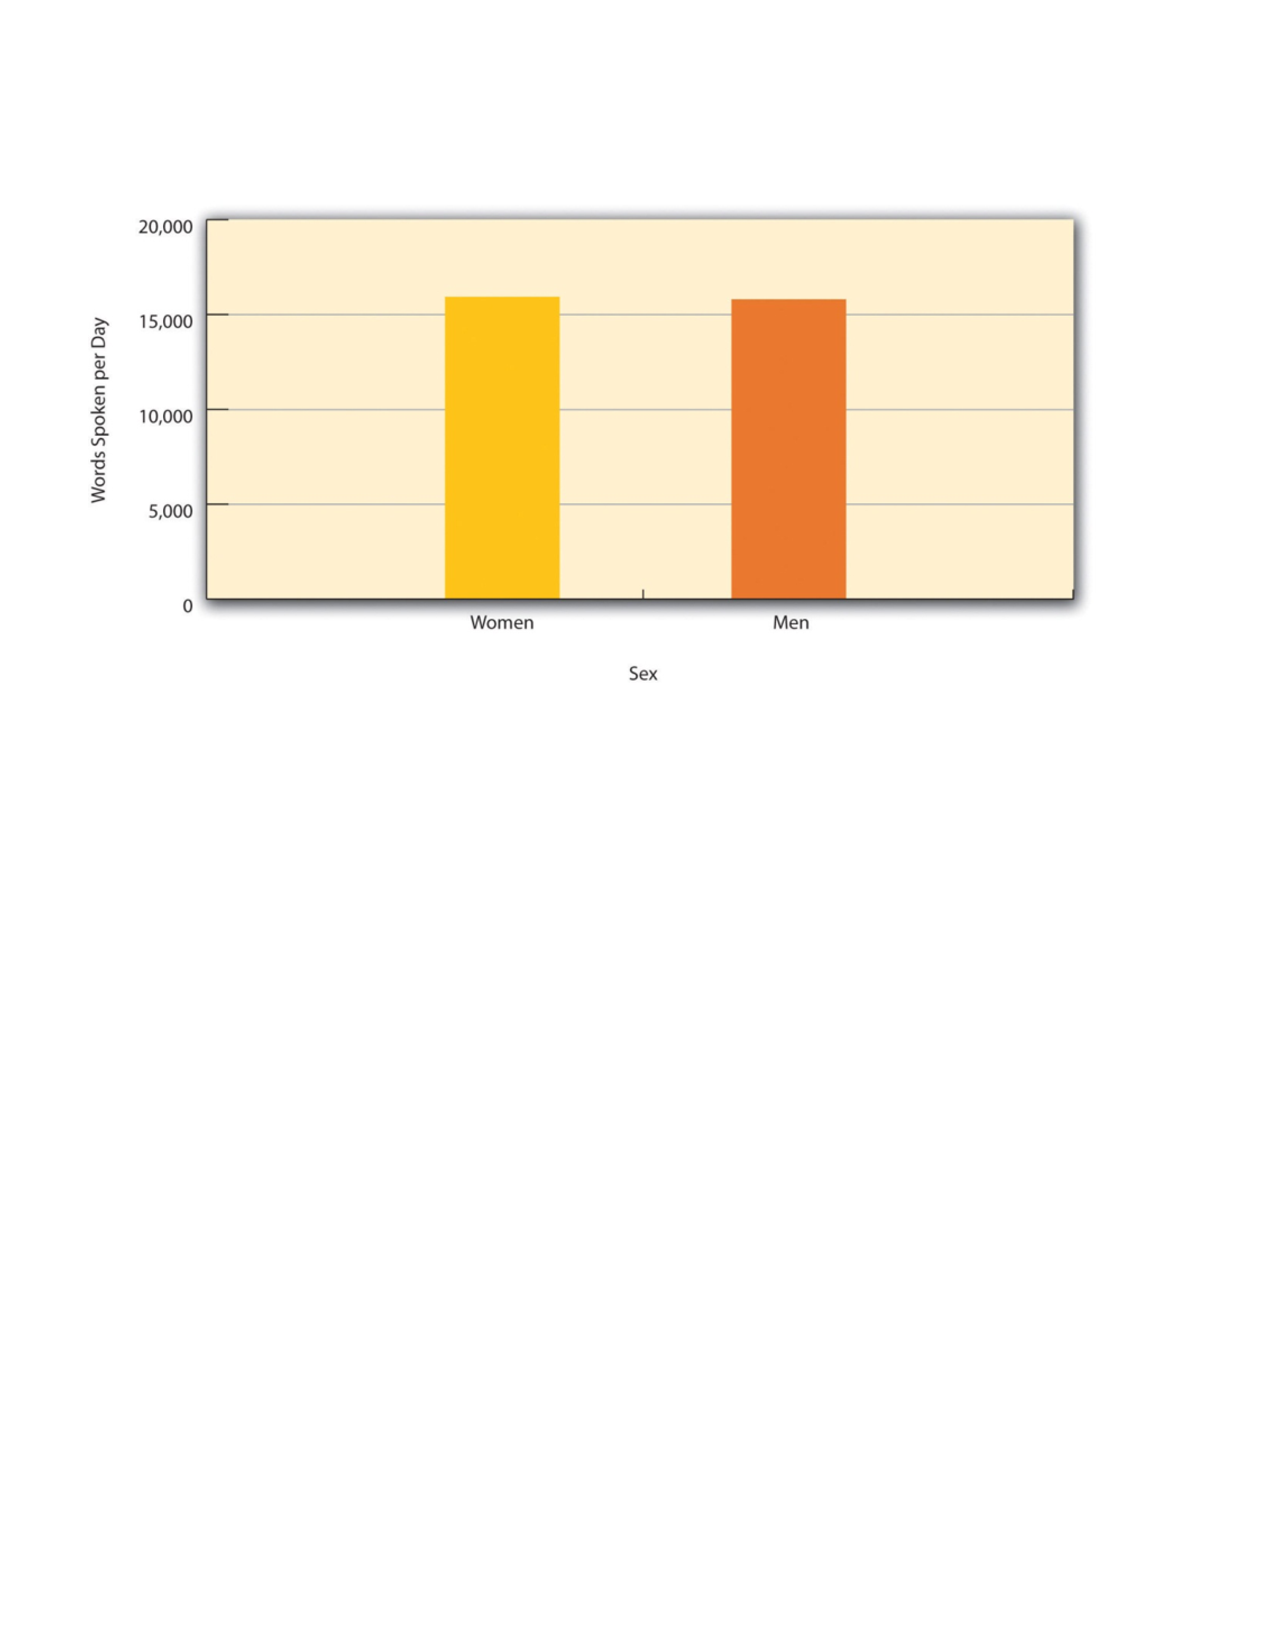
\includegraphics{figures/C2F2_barchart.pdf}
\caption{Bar Graph Showing the Very Small Difference in the Mean Number
of Words Spoken per Day by Women and Men in a Large Sample. Based on
data from ``Are Women Really More Talkative Than Men?'' by M. R. Mehl,
S. Vazire, N. Ramirez-Esparza, R. B. Slatcher, and J. W. Pennebaker,
2007, Science, 317, p.~82.}
\end{figure}

{[}fig:Bargraph{]}

Differences between groups are usually described by giving the mean
score and standard deviation for each group. This information can also
be presented in a bar graph like that in Figure 2.1, where the heights
of the bars represent the group means.

\subsection{Correlations Between Quantitative
Variables}\label{correlations-between-quantitative-variables}

A second basic form of statistical relationship is a correlation between
two quantitative variables, where the average score on one variable
differs systematically across the levels of the other. Again, a wide
variety of research questions in psychology take this form. Is being a
happier person associated with being more talkative? Do people who are
narcissistic tend to take more selfies? Does the effectiveness of
psychotherapy depend on how much the patient likes the therapist?

\begin{figure}[htbp]
\centering
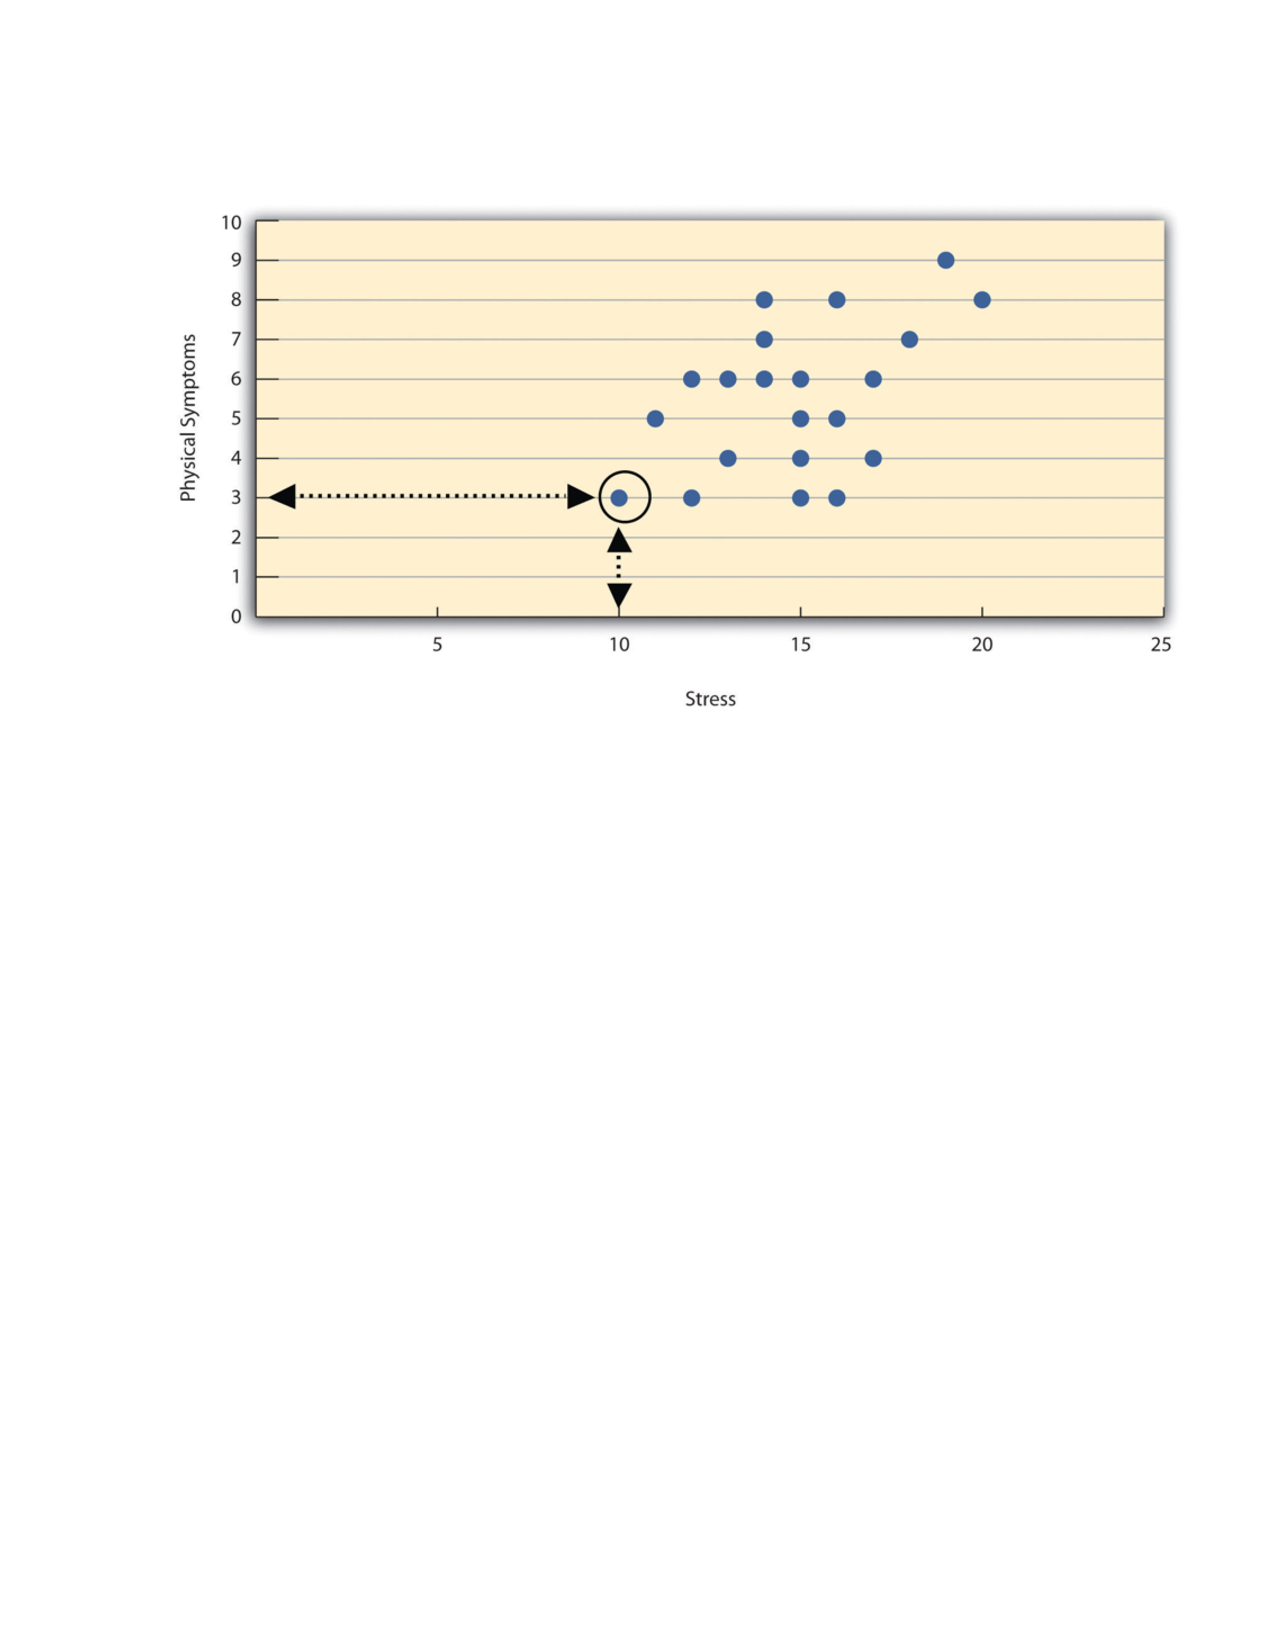
\includegraphics{figures/C2F3Correlation.pdf}
\caption{Scatterplot Showing a Hypothetical Positive Relationship
Between Stress and Number of Physical Symptoms. The circled point
represents a person whose stress score was 10 and who had three physical
symptoms. Pearson's r for these data is +.51.}
\end{figure}

{[}fig:Correlation{]}

Correlations between quantitative variables are often presented using
scatterplots. Figure 2.2 shows some hypothetical data on the
relationship between the amount of stress people are under and the
number of physical symptoms they have. Each point in the scatterplot
represents one person's score on both variables. For example, the
circled point in Figure 2.2 represents a person whose stress score was
10 and who had three physical symptoms. Taking all the points into
account, one can see that people under more stress tend to have more
physical symptoms. This is a good example of a positive relationship, in
which higher scores on one variable tend to be associated with higher
scores on the other. A negative relationship is one in which higher
scores on one variable tend to be associated with lower scores on the
other. There is a negative relationship between stress and immune system
functioning, for example, because higher stress is associated with lower
immune system functioning.

\begin{figure}[htbp]
\centering
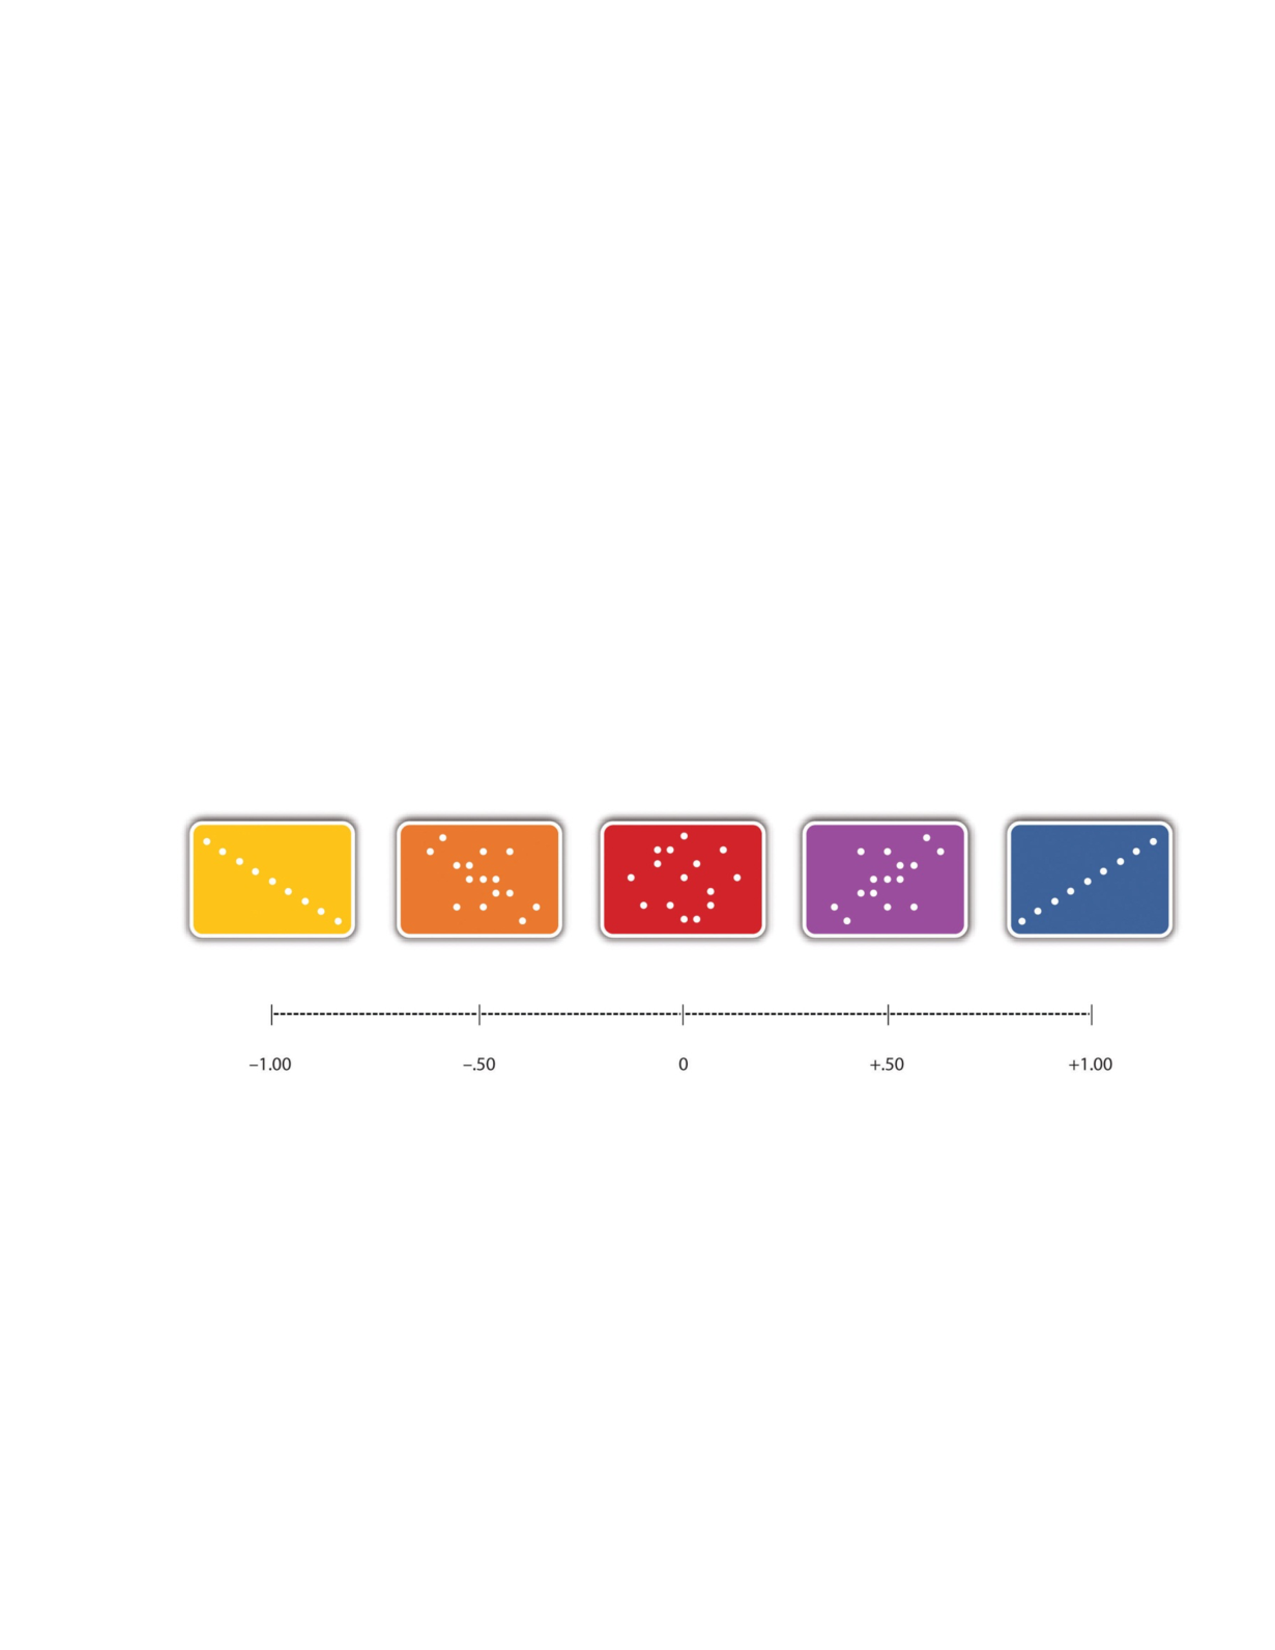
\includegraphics{figures/C2F4Correlation2.pdf}
\caption{image}
\end{figure}

{[}fig:Correlation2{]}

The strength of a correlation between quantitative variables is
typically measured using a statistic called Pearson's r. As Figure 2.3
shows, Pearson's r ranges from −1.00 (the strongest possible negative
relationship) to +1.00 (the strongest possible positive relationship). A
value of 0 means there is no relationship between the two variables.
When Pearson's r is 0, the points on a scatterplot form a shapeless
``cloud.'' As its value moves toward −1.00 or +1.00, the points come
closer and closer to falling on a single straight line. The website
\url{http://rpsychologist.com/d3/correlation/}, created by Kristoffer
Magnusson, provides an excellent interactive visualization of
correlations that permits you to adjust the strength and direction of a
correlation while witnessing the corresponding changes to the
scatterplot.

Pearson's r is a good measure only for linear relationships, in which
the points are best approximated by a straight line. It is not a good
measure for nonlinear relationships, in which the points are better
approximated by a curved line. Figure 2.4, for example, shows a
hypothetical relationship between the amount of sleep people get per
night and their level of depression. In this example, the line that best
approximates the points is a curve---a kind of upside- down
``U''---because people who get about eight hours of sleep tend to be the
least depressed. Those who get too little sleep and those who get too
much sleep tend to be more depressed. Nonlinear relationships are fairly
common in psychology, but measuring their strength is beyond the scope
of this book.

\subsection{Correlation Does Not Imply
Causation}\label{correlation-does-not-imply-causation}

\begin{figure}[htbp]
\centering
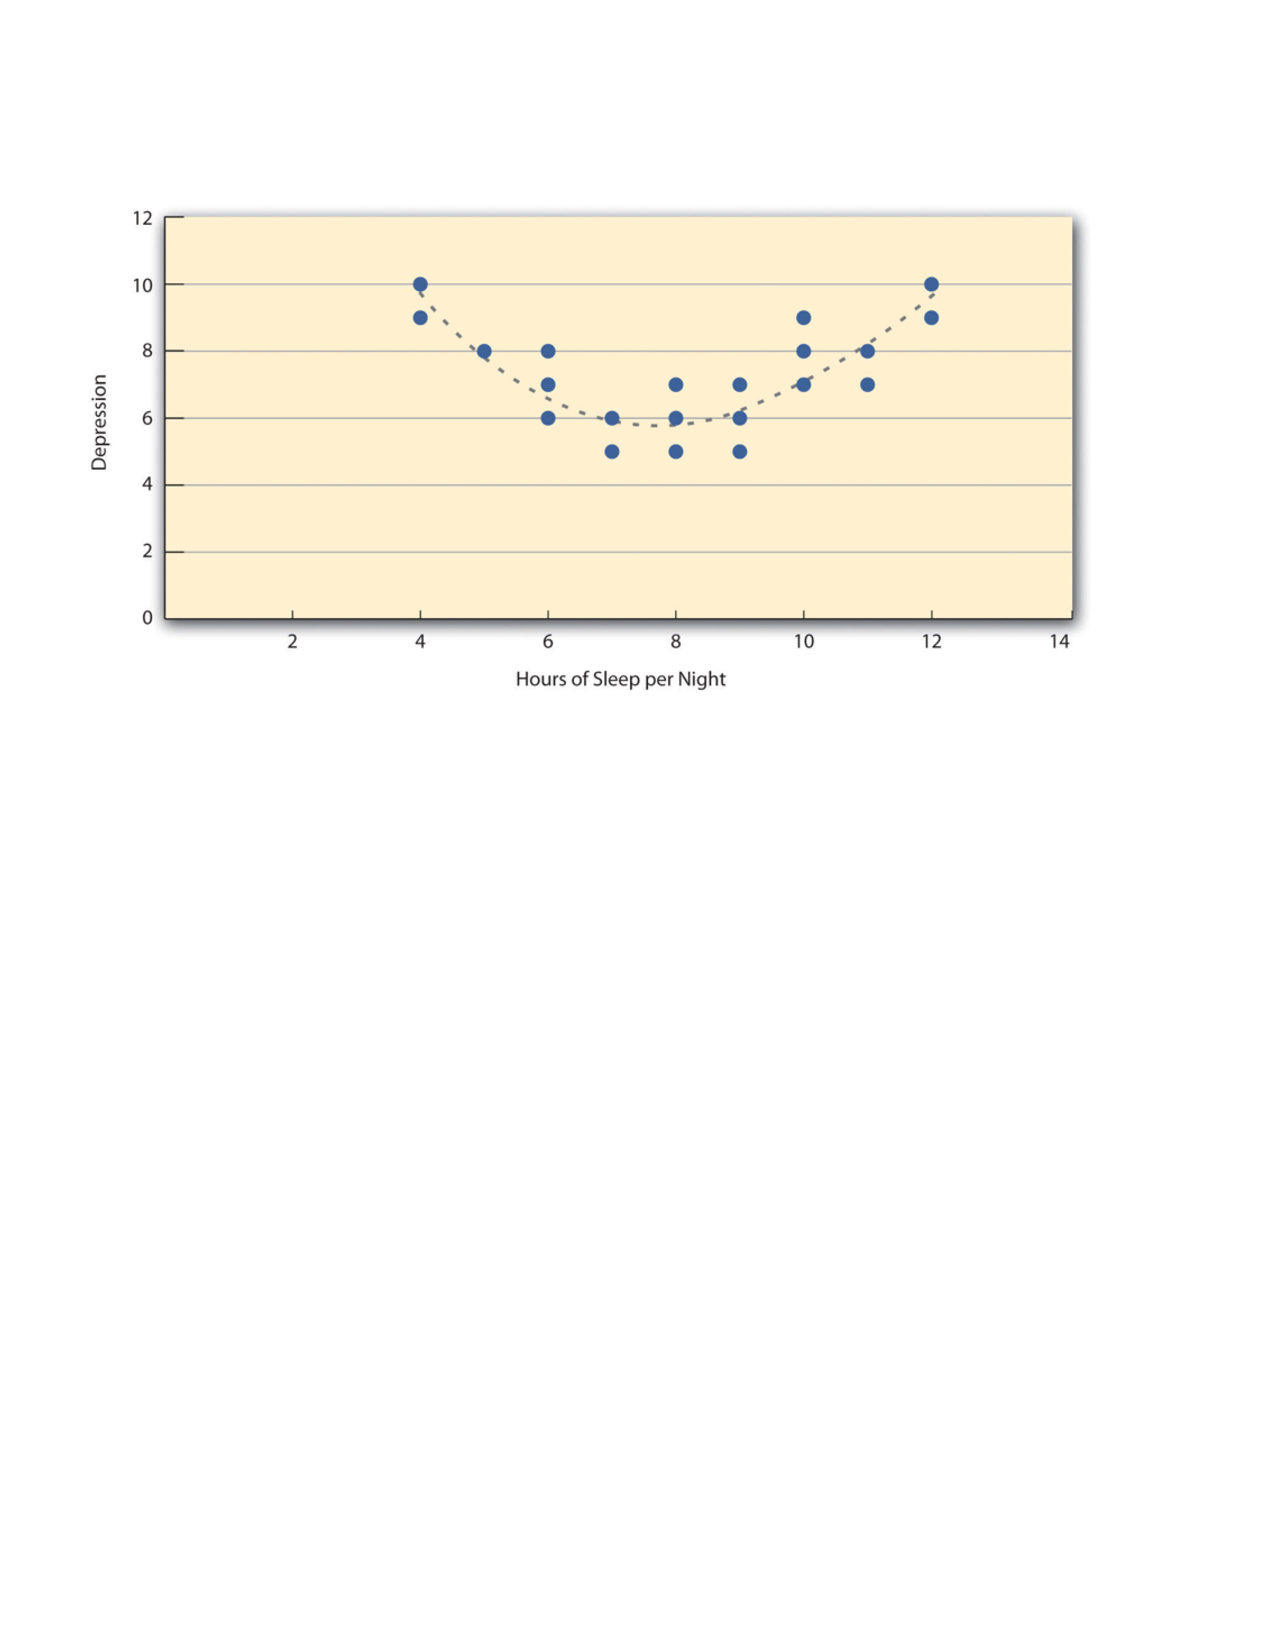
\includegraphics{figures/C2F5Ucurve.pdf}
\caption{Hypothetical Nonlinear Relationship Between Sleep and
Depression}
\end{figure}

{[}fig:Nonlinear{]}

Researchers are often interested in a statistical relationship between
two variables because they think that one of the variables causes the
other. That is, the statistical relationship reflects a causal
relationship. In these situations, the variable that is thought to be
the cause is called the independent variable (often referred to as X for
short), and the variable that is thought to be the effect is called the
dependent variable (often referred to as Y). For example, the
statistical relationship between whether or not a depressed person
receives psychotherapy and the number of depressive symptoms he or she
has reflects the fact that the psychotherapy (the independent variable)
causes the reduction in symptoms (the dependent variable). Understanding
causal relationships is important in part because it allows us to change
people's behavior in predictable ways. If we know that psychotherapy
causes a reduction in depressive symptoms---and we want people to have
fewer depressive symptoms---then we can use psychotherapy to achieve
this goal.

But not all statistical relationships reflect causal relationships. This
is what psychologists mean when they say, ``Correlation does not imply
causation.'' An amusing example of this comes from a 2012 study that
showed a positive correlation (Pearson's r = 0.79) between the per
capita chocolate consumption of a nation and the number of Nobel prizes
awarded to citizens of that nation1. It seems clear, however, that this
does not mean that eating chocolate causes people to win Nobel prizes,
and it would not make sense to try to increase the number of Nobel
prizes won by recommending that parents feed their children more
chocolate.

There are two reasons that correlation does not imply causation. The
first is called the directionality problem. Two variables, X and Y, can
be statistically related because X causes Y or because Y causes X.
Consider, for example, a study showing that whether or not people
exercise is statistically related to how happy they are---such that
people who exercise are happier on average than people who do not. This
statistical relationship is consistent with the idea that exercising
causes happiness, but it is also consistent with the idea that happiness
causes exercise. Perhaps being happy gives people more energy or leads
them to seek opportunities to socialize with others by going to the gym.
The second reason that correlation does not imply causation is called
the third-variable problem. Two variables, X and Y, can be statistically
related not because X causes Y, or because Y causes X, but because some
third variable, Z, causes both X and Y. For example, the fact that
nations that have won more Nobel prizes tend to have higher chocolate
consumption probably reflects geography in that European countries tend
to have higher rates of per capita chocolate consumption and invest more
in education and technology (once again, per capita) than many other
countries in the world. Similarly, the statistical relationship between
exercise and happiness could mean that some third variable, such as
physical health, causes both of the others. Being physically healthy
could cause people to exercise and cause them to be happier.

\begin{figure}[htbp]
\centering
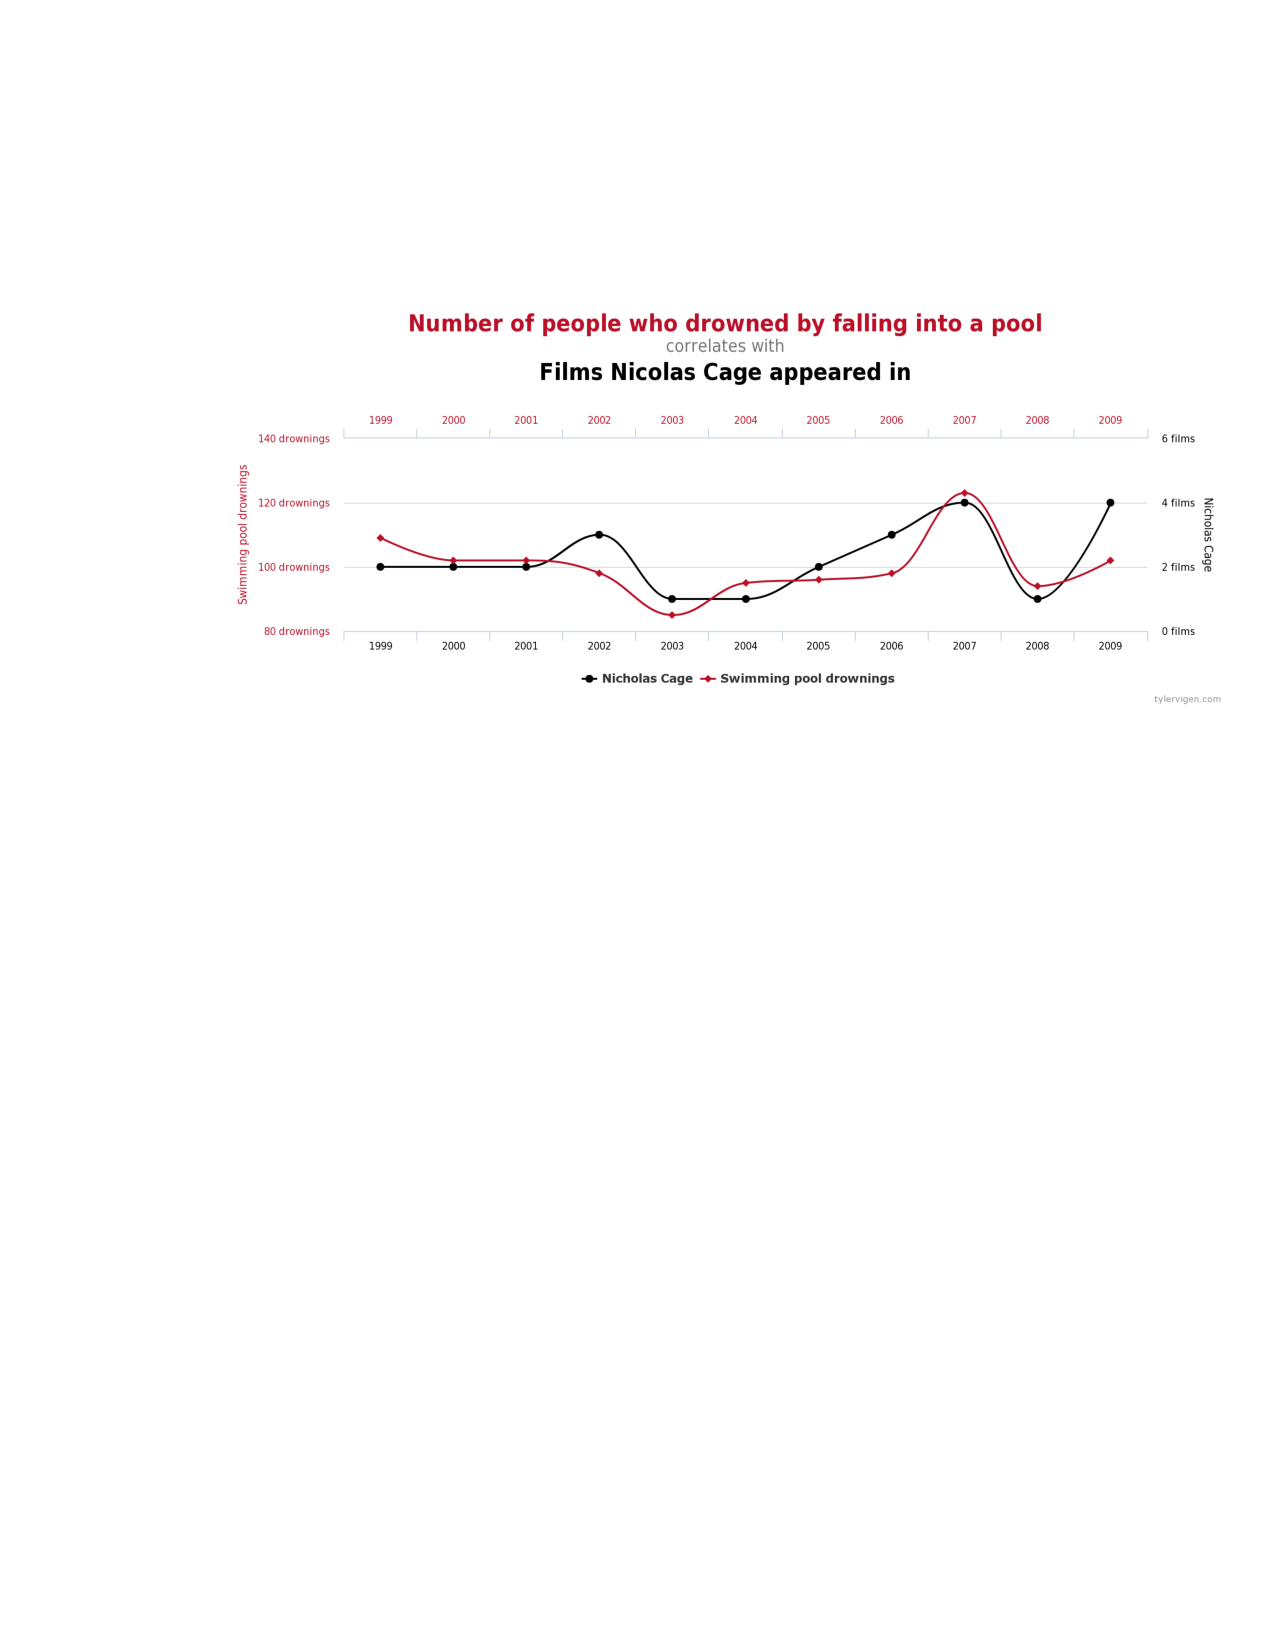
\includegraphics{figures/C2F6NickCage.pdf}
\caption{For some excellent and funny examples of correlations that
almost certainly do not show causation, enjoy the strange correlations
found at \url{http://www.tylervigen.com}}
\end{figure}

{[}fig:NickCage{]}

\subsection{\texorpdfstring{``Lots of Candy Could Lead to
Violence''}{Lots of Candy Could Lead to Violence}}\label{lots-of-candy-could-lead-to-violence}

Although researchers in psychology know that correlation does not imply
causation, many journalists do not. One website about correlation and
causation,
\href{http://jonathan.mueller.faculty.noctrl.edu/100/\%20correlation_or_causation.htm}{http://jonathan.mueller.faculty.noctrl.edu/100/
correlation\_or\_causation.htm}, links to dozens of media reports about
real biomedical and psychological research. Many of the headlines
suggest that a causal relationship has been demonstrated, when a careful
reading of the articles shows that it has not because of the
directionality and third-variable problems.

One such article is about a study showing that children who ate candy
every day were more likely than other children to be arrested for a
violent offense later in life. But could candy really ``lead to''
violence, as the headline suggests? What alternative explanations can
you think of for this statistical relationship? How could the headline
be rewritten so that it is not misleading?

As we will see later in the book, there are various ways that
researchers address the directionality and third-variable problems. The
most effective, however, is to conduct an experiment. An experiment is a
study in which the researcher manipulates the independent variable. For
example, instead of simply measuring how much people exercise, a
researcher could bring people into a laboratory and randomly assign half
of them to run on a treadmill for 15 minutes and the rest to sit on a
couch for 15 minutes. Although this seems like a minor change to the
research design, it is extremely important. Now if the exercisers end up
in more positive moods than those who did not exercise, it cannot be
because their moods affected how much they exercised (because it was the
researcher who determined how much they exercised). Likewise, it cannot
be because some third variable (e.g., physical health) affected both how
much they exercised and what mood they were in (because, again, it was
the researcher who determined how much they exercised). Thus experiments
eliminate the directionality and third-variable problems and allow
researchers to draw firm conclusions about causal relationships. We will
have much more to say about experimental and nonexperimental research
later in the book.

\subsection{Key Takeaways}\label{key-takeaways-4}

\begin{itemize}
\item
  Research questions in psychology are about variables and relationships
  between variables.
\item
  Two basic forms of statistical relationship are differences between
  group means and correlations between quantitative variables, each of
  which can be described using a few simple statistical techniques.
\item
  Correlation does not imply causation. A statistical relationship
  between two variables, X and Y, does not necessarily mean that X
  causes Y. It is also possible that Y causes X, or that a third
  variable, Z, causes both X and Y.
\end{itemize}

\subsection{Exercises}\label{exercises-4}

\begin{enumerate}
\def\labelenumi{\arabic{enumi}.}
\item
  Practice: List 10 variables that might be of interest to a researcher
  in psychology. For each, specify whether it is quantitative or
  categorical.
\item
  Practice: Imagine that you categorize people as either introverts
  (quieter, shyer, more inward looking) or extraverts (louder, more
  outgoing, more outward looking). Sketch a bar graph showing a
  hypothetical statistical relationship between this variable and the
  number of words people speak per day.
\item
  Practice: Now imagine that you measure people's levels of extraversion
  as a quantitative variable, with values ranging from 0 (extreme
  introversion) to 30 (extreme extraversion). Sketch a scatterplot
  showing a hypothetical statistical relationship between this variable
  and the number of words people speak per day.
\item
  Practice: For each of the following statistical relationships, decide
  whether the directionality problem is present and think of at least
  one plausible third variable:

  \begin{itemize}
  \item
    People who eat more lobster tend to live longer.
  \item
    People who exercise more tend to weigh less.
  \item
    College students who drink more alcohol tend to have poorer grades.
  \end{itemize}
\end{enumerate}

\section{Generating Good Research
Questions}\label{generating-good-research-questions}

Good research must begin with a good research question. Yet coming up
with good research questions is something that novice researchers often
find difficult and stressful. One reason is that this is a creative
process that can appear mysterious---even magical---with experienced
researchers seeming to pull interesting research questions out of thin
air. However, psychological research on creativity has shown that it is
neither as mysterious nor as magical as it appears. It is largely the
product of ordinary thinking strategies and persistence (Weisberg,
1993). This section covers some fairly simple strategies for finding
general research ideas, turning those ideas into empirically testable
research questions, and finally evaluating those questions in terms of
how interesting they are and how feasible they would be to answer.

\subsection{Finding Inspiration}\label{finding-inspiration}

Research questions often begin as more general research ideas---usually
focusing on some behavior or psychological characteristic:
talkativeness, learning, depression, bungee jumping, and so on. Before
looking at how to turn such ideas into empirically testable research
questions, it is worth looking at where such ideas come from in the
first place. Three of the most common sources of inspiration are
informal observations, practical problems, and previous research.

Informal observations include direct observations of our own and others'
behavior as well as secondhand observations from nonscientific sources
such as newspapers, books, blogs, and so on. For example, you might
notice that you always seem to be in the slowest moving line at the
grocery store. Could it be that most people think the same thing? Or you
might read in a local newspaper about people donating money and food to
a local family whose house has burned down and begin to wonder about who
makes such donations and why. Some of the most famous research in
psychology has been inspired by informal observations. Stanley Milgram's
famous research on obedience to authority, for example, was inspired in
part by journalistic reports of the trials of accused Nazi war
criminals---many of whom claimed that they were only obeying orders.
This led him to wonder about the extent to which ordinary people will
commit immoral acts simply because they are ordered to do so by an
authority figure (Milgram, 1963).

Practical problems can also inspire research ideas, leading directly to
applied research in such domains as law, health, education, and sports.
Does taking lecture notes by hand improve students' exam performance?
How effective is psychotherapy for depression compared to drug therapy?
To what extent do cell phones impair people's driving ability? How can
we teach children to read more efficiently? What is the best mental
preparation for running a marathon?

Probably the most common inspiration for new research ideas, however, is
previous research. Recall that science is a kind of large-scale
collaboration in which many different researchers read and evaluate each
other's work and conduct new studies to build on it. Of course,
experienced researchers are familiar with previous research in their
area of expertise and probably have a long list of ideas. This suggests
that novice researchers can find inspiration by consulting with a more
experienced researcher (e.g., students can consult a faculty member).
But they can also find inspiration by picking up a copy of almost any
professional journal and reading the titles and abstracts. In one
typical issue of Psychological Science, for example, you can find
articles on the perception of shapes, anti-Semitism, police lineups, the
meaning of death, second-language learning, people who seek negative
emotional experiences, and many other topics. If you can narrow your
interests down to a particular topic (e.g., memory) or domain (e.g.,
health care), you can also look through more specific journals, such as
Memory \& Cognition or Health Psychology.

\subsection{Generating Empirically Testable Research
Questions}\label{generating-empirically-testable-research-questions}

Once you have a research idea, you need to use it to generate one or
more empirically testable research questions, that is, questions
expressed in terms of a single variable or relationship between
variables. One way to do this is to look closely at the discussion
section in a recent research article on the topic. This is the last
major section of the article, in which the researchers summarize their
results, interpret them in the context of past research, and suggest
directions for future research. These suggestions often take the form of
specific research questions, which you can then try to answer with
additional research. This can be a good strategy because it is likely
that the suggested questions have already been identified as interesting
and important by experienced researchers.

But you may also want to generate your own research questions. How can
you do this? First, if you have a particular behavior or psychological
characteristic in mind, you can simply conceptualize it as a variable
and ask how frequent or intense it is. How many words on average do
people speak per day? How accurate are our memories of traumatic events?
What percentage of people have sought professional help for depression?
If the question has never been studied scientifically---which is
something that you will learn in your literature review---then it might
be interesting and worth pursuing.

If scientific research has already answered the question of how frequent
or intense the behavior or characteristic is, then you should consider
turning it into a question about a statistical relationship between that
behavior or characteristic and some other variable. One way to do this
is to ask yourself the following series of more general questions and
write down all the answers you can think of.

\begin{itemize}
\item
  What are some possible causes of the behavior or characteristic?
\item
  What are some possible effects of the behavior or characteristic?
\item
  What types of people might exhibit more or less of the behavior or
  characteristic?
\item
  What types of situations might elicit more or less of the behavior or
  characteristic?
\end{itemize}

In general, each answer you write down can be conceptualized as a second
variable, suggesting a question about a statistical relationship. If you
were interested in talkativeness, for example, it might occur to you
that a possible cause of this psychological characteristic is family
size. Is there a statistical relationship between family size and
talkativeness? Or it might occur to you that people seem to be more
talkative in same-sex groups than mixed-sex groups. Is there a
difference in the average level of talkativeness of people in same-sex
groups and people in mixed- sex groups? This approach should allow you
to generate many different empirically testable questions about almost
any behavior or psychological characteristic.

If through this process you generate a question that has never been
studied scientifically---which again is something that you will learn in
your literature review---then it might be interesting and worth
pursuing. But what if you find that it has been studied scientifically?
Although novice researchers often want to give up and move on to a new
question at this point, this is not necessarily a good strategy. For one
thing, the fact that the question has been studied scientifically and
the research published suggests that it is of interest to the scientific
community. For another, the question can almost certainly be refined so
that its answer will still contribute something new to the research
literature. Again, asking yourself a series of more general questions
about the statistical relationship is a good strategy.

\begin{itemize}
\item
  Are there other ways to operationally define the variables?
\item
  Are there types of people for whom the statistical relationship might
  be stronger or weaker?
\item
  Are there situations in which the statistical relationship might be
  stronger or weaker---including situations with practical importance?
\end{itemize}

For example, research has shown that women and men speak about the same
number of words per day---but this was when talkativeness was measured
in terms of the number of words spoken per day among university students
in the United States and Mexico. We can still ask whether other ways of
measuring talkativeness---perhaps the number of different people spoken
to each day---produce the same result. Or we can ask whether studying
elderly people or people from other cultures produces the same result.
Again, this approach should help you generate many different research
questions about almost any statistical relationship.

\subsection{Evaluating Research
Questions}\label{evaluating-research-questions}

Researchers usually generate many more research questions than they ever
attempt to answer. This means they must have some way of evaluating the
research questions they generate so that they can choose which ones to
pursue. In this section, we consider two criteria for evaluating
research questions: the interestingness of the question and the
feasibility of answering it.

\subsection{Interestingness}\label{interestingness}

How often do people tie their shoes? Do people feel pain when you punch
them in the jaw? Are women more likely to wear makeup than men? Do
people prefer vanilla or chocolate ice cream? Although it would be a
fairly simple matter to design a study and collect data to answer these
questions, you probably would not want to because they are not
interesting. We are not talking here about whether a research question
is interesting to us personally but whether it is interesting to people
more generally and, especially, to the scientific community. But what
makes a research question interesting in this sense? Here we look at
three factors that affect the interestingness of a research question:

\begin{itemize}
\item
  the answer is in doubt
\item
  the answer fills a gap in the research literature
\item
  the answer has important practical implications.
\end{itemize}

First, a research question is interesting to the extent that its answer
is in doubt. Obviously, questions that have been answered by scientific
research are no longer interesting as the subject of new empirical
research. But the fact that a question has not been answered by
scientific research does not necessarily make it interesting. There has
to be some reasonable chance that the answer to the question will be
something that we did not already know. But how can you assess this
before actually collecting data? One approach is to try to think of
reasons to expect different answers to the question---especially ones
that seem to conflict with common sense. If you can think of reasons to
expect at least two different answers, then the question might be
interesting. If you can think of reasons to expect only one answer, then
it probably is not. The question of whether women are more talkative
than men is interesting because there are reasons to expect both
answers. The existence of the stereotype itself suggests the answer
could be yes, but the fact that women's and men's verbal abilities are
fairly similar suggests the answer could be no. The question of whether
people feel pain when you punch them in the jaw is not interesting
because there is absolutely no reason to think that the answer could be
anything other than a resounding yes.

A second important factor to consider when deciding if a research
question is interesting is whether answering it will fill a gap in the
research literature. Again, this means in part that the question has not
already been answered by scientific research. But it also means that the
question is in some sense a natural one for people who are familiar with
the research literature. For example, the question of whether taking
lecture notes by hand can help improve students' exam performance would
be likely to occur to anyone who was familiar with research on note
taking and the ineffectiveness of shallow processing on learning.

A final factor to consider when deciding whether a research question is
interesting is whether its answer has important practical implications.
Again, the question of whether taking notes by hand improves learning
has important implications for education, including classroom policies
concerning technology use. The question of whether cell phone use
impairs driving is interesting because it is relevant to the personal
safety of everyone who travels by car and to the debate over whether
cell phone use should be restricted by law.

\subsection{Feasibility}\label{feasibility}

A second important criterion for evaluating research questions is the
feasibility of successfully answering them. There are many factors that
affect feasibility, including time, money, equipment and materials,
technical knowledge and skill, and access to research participants.
Clearly, researchers need to take these factors into account so that
they do not waste time and effort pursuing research that they cannot
complete successfully.

Looking through a sample of professional journals in psychology will
reveal many studies that are complicated and difficult to carry out.
These include longitudinal designs in which participants are tracked
over many years, neuroimaging studies in which participants' brain
activity is measured while they carry out various mental tasks, and
complex non-experimental studies involving several variables and
complicated statistical analyses. Keep in mind, though, that such
research tends to be carried out by teams of highly trained researchers
whose work is often supported in part by government and private grants.
Keep in mind also that research does not have to be complicated or
difficult to produce interesting and important results. Looking through
a sample of professional journals will also reveal studies that are
relatively simple and easy to carry out---perhaps involving a
convenience sample of university students and a paper-and-pencil task.

A final point here is that it is generally good practice to use methods
that have already been used successfully by other researchers. For
example, if you want to manipulate people's moods to make some of them
happy, it would be a good idea to use one of the many approaches that
have been used successfully by other researchers (e.g., paying them a
compliment). This is good not only for the sake of feasibility---the
approach is ``tried and true''---but also because it provides greater
continuity with previous research. This makes it easier to compare your
results with those of other researchers and to understand the
implications of their research for yours, and vice versa.

\subsection{Key takeaways}\label{key-takeaways-5}

\begin{itemize}
\item
  Research ideas can come from a variety of sources, including informal
  observations, practical problems, and previous research.
\item
  Research questions expressed in terms of variables and relationships
  between variables can be suggested by other researchers or generated
  by asking a series of more general questions about the behavior or
  psychological characteristic of interest.
\item
  It is important to evaluate how interesting a research question is
  before designing a study and collecting data to answer it. Factors
  that affect interestingness are the extent to which the answer is in
  doubt, whether it fills a gap in the research literature, and whether
  it has important practical implications.
\item
  It is also important to evaluate how feasible a research question will
  be to answer. Factors that affect feasibility include time, money,
  technical knowledge and skill, and access to special equipment and
  research participants.
\end{itemize}

\subsection{Exercises}\label{exercises-5}

\begin{enumerate}
\def\labelenumi{\arabic{enumi}.}
\item
  Practice: Generate five research ideas based on each of the following:
  informal observations, practical problems, and topics discussed in
  recent issues of professional journals.
\item
  Practice: Generate five empirical research questions about each of the
  following behaviors or psychological characteristics: long-distance
  running, getting tattooed, social anxiety, bullying, and memory for
  early childhood events.
\item
  Practice: Evaluate each of the research questions you generated in
  Exercise 2 in terms of its interestingness based on the criteria
  discussed in this section.
\item
  Practice: Find an issue of a journal that publishes short empirical
  research reports (e.g., Psychological Science, Psychonomic Bulletin
  and Review, Personality and Social Psychology Bulletin). Pick three
  studies, and rate each one in terms of how feasible it would be for
  you to replicate it with the resources available to you right now. Use
  the following rating scale: (1) You could replicate it essentially as
  reported. (2) You could replicate it with some simplifications. (3)
  You could not replicate it. Explain each rating.
\end{enumerate}

\section{Reviewing the Research
Literature}\label{reviewing-the-research-literature}

Reviewing the research literature means finding, reading, and
summarizing the published research relevant to your question. An
empirical research report written in American Psychological Association
(APA) style always includes a written literature review, but it is
important to review the literature early in the research process for
several reasons.

\begin{itemize}
\item
  It can help you turn a research idea into an interesting research
  question.
\item
  It can tell you if a research question has already been answered.
\item
  It can help you evaluate the interestingness of a research question.
\item
  It can give you ideas for how to conduct your own study.
\item
  It can tell you how your study fits into the research literature.
\end{itemize}

\subsection{What Is the Research
Literature?}\label{what-is-the-research-literature}

The research literature in any field is all the published research in
that field. The research literature in psychology is
enormous---including millions of scholarly articles and books dating to
the beginning of the field---and it continues to grow. Although its
boundaries are somewhat fuzzy, the research literature definitely does
not include self-help and other pop psychology books, dictionary and
encyclopedia entries, websites, and similar sources that are intended
mainly for the general public. These are considered unreliable because
they are not reviewed by other researchers and are often based on little
more than common sense or personal experience. Wikipedia contains much
valuable information, but the fact that its authors are anonymous and
may not have any formal training or expertise in that subject area, and
its content continually changes makes it unsuitable as a basis of sound
scientific research. For our purposes, it helps to define the research
literature as consisting almost entirely of two types of sources:
articles in professional journals, and scholarly books in psychology and
related fields.

\subsection{Professional Journals}\label{professional-journals}

Professional journals are periodicals that publish original research
articles. There are thousands of professional journals that publish
research in psychology and related fields. They are usually published
monthly or quarterly in individual issues, each of which contains
several articles. The issues are organized into volumes, which usually
consist of all the issues for a calendar year. Some journals are
published in hard copy only, others in both hard copy and electronic
form, and still others in electronic form only.

Most articles in professional journals are one of two basic types:
empirical research reports and review articles. Empirical research
reports describe one or more new empirical studies conducted by the
authors. They introduce a research question, explain why it is
interesting, review previous research, describe their method and
results, and draw their conclusions. Review articles summarize
previously published research on a topic and usually present new ways to
organize or explain the results. When a review article is devoted
primarily to presenting a new theory, it is often referred to as a
theoretical article.

Most professional journals in psychology undergo a process of
double-blind peer review. Researchers who want to publish their work in
the journal submit a manuscript to the editor---who is generally an
established researcher too---who in turn sends it to two or three
experts on the topic. Each reviewer reads the manuscript, writes a
critical but constructive review, and sends the review back to the
editor along with his or her recommendations. The editor then decides
whether to accept the article for publication, ask the authors to make
changes and resubmit it for further consideration, or reject it
outright. In any case, the editor forwards the reviewers' written
comments to the researchers so that they can revise their manuscript
accordingly. This entire process is double-blind, as the reviewers do
not know the identity of the researcher(s), and vice versa. Double-blind
peer review is helpful because it ensures that the work meets basic
standards of the field before it can enter the research literature.
However, in order to increase transparency and accountability some newer
open access journals (e.g., Frontiers in Psychology) utilize an open
peer review process wherein the identities of the reviewers (which
remain concealed during the peer review process) are published alongside
the journal article.

\subsection{Scholarly Books}\label{scholarly-books}

Scholarly books are books written by researchers and practitioners
mainly for use by other researchers and practitioners. A monograph is
written by a single author or a small group of authors and usually gives
a coherent presentation of a topic much like an extended review article.
Edited volumes have an editor or a small group of editors who recruit
many authors to write separate chapters on different aspects of the same
topic. Although edited volumes can also give a coherent presentation of
the topic, it is not unusual for each chapter to take a different
perspective or even for the authors of different chapters to openly
disagree with each other. In general, scholarly books undergo a peer
review process similar to that used by professional journals.

\subsection{Literature Search
Strategies}\label{literature-search-strategies}

\subsection{Using PsycINFO and Other
Databases}\label{using-psycinfo-and-other-databases}

The primary method used to search the research literature involves using
one or more electronic databases. These include Academic Search Premier,
JSTOR, and ProQuest for all academic disciplines, ERIC for education,
and PubMed for medicine and related fields. The most important for our
purposes, however, is PsycINFO, which is produced by the APA. PsycINFO
is so comprehensive---covering thousands of professional journals and
scholarly books going back more than 100 years---that for most purposes
its content is synonymous with the research literature in psychology.
Like most such databases, PsycINFO is usually available through your
university library.

PsycINFO consists of individual records for each article, book chapter,
or book in the database. Each record includes basic publication
information, an abstract or summary of the work (like the one presented
at the start of this chapter), and a list of other works cited by that
work. A computer interface allows entering one or more search terms and
returns any records that contain those search terms. (These interfaces
are provided by different vendors and therefore can look somewhat
different depending on the library you use.) Each record also contains
lists of keywords that describe the content of the work and also a list
of index terms. The index terms are especially helpful because they are
standardized. Research on differences between women and men, for
example, is always indexed under ``Human Sex Differences.'' Research on
notetaking is always indexed under the term ``Learning Strategies.'' If
you do not know the appropriate index terms, PsycINFO includes a
thesaurus that can help you find them.

Given that there are nearly four million records in PsycINFO, you may
have to try a variety of search terms in different combinations and at
different levels of specificity before you find what you are looking
for. Imagine, for example, that you are interested in the question of
whether women and men differ in terms of their ability to recall
experiences from when they were very young. If you were to enter
``memory for early experiences'' as your search term, PsycINFO would
return only six records, most of which are not particularly relevant to
your question. However, if you were to enter the search term ``memory,''
it would return 149,777 records---far too many to look through
individually. This is where the thesaurus helps. Entering ``memory''
into the thesaurus provides several more specific index terms---one of
which is ``early memories.'' While searching for ``early memories''
among the index terms returns 1,446 records---still too many too look
through individually---combining it with ``human sex differences'' as a
second search term returns 37 articles, many of which are highly
relevant to the topic.

Depending on the vendor that provides the interface to PsycINFO, you may
be able to save, print, or e-mail the relevant PsycINFO records. The
records might even contain links to full-text copies of the works
themselves.

\subsection{Using Other Search
Techniques}\label{using-other-search-techniques}

In addition to entering search terms into PsycINFO and other databases,
there are several other techniques you can use to search the research
literature. First, if you have one good article or book chapter on your
topic---a recent review article is best---you can look through the
reference list of that article for other relevant articles, books, and
book chapters. In fact, you should do this with any relevant article or
book chapter you find. You can also start with a classic article or book
chapter on your topic, find its record in PsycINFO (by entering the
author's name or article's title as a search term), and link from there
to a list of other works in PsycINFO that cite that classic article.
This works because other researchers working on your topic are likely to
be aware of the classic article and cite it in their own work. You can
also do a general Internet search using search terms related to your
topic or the name of a researcher who conducts research on your topic.
This might lead you directly to works that are part of the research
literature (e.g., articles in open-access journals or posted on
researchers' own websites).

\subsection{Google Scholar}\label{google-scholar}

The search engine Google Scholar \url{https://scholar.google.com} is
especially useful alternative to PsycInfo and other databases. Many
researchers rely almost exclusively on Google Scholar because you it
maintains a comprehensive list of nearly all published work in all
fields, including Psychology. It's also easier to search and navigate
that many other databases.

Google scholar has lots of useful features for finding articles that can
be relevant to you. You can enter any search term in, and Google Scholar
will find things related to your keywords. It's good to start with your
research topic, but if you are looking for a specific paper then you can
enter the title (or part of the title), or the authors and the year. Try
it out.

\begin{figure}[htbp]
\centering

\includegraphics{figures/CrumpPlosOne.png}
\caption{image}
\end{figure}

{[}fig:PlosOne{]}

The figure above shows an example of paper listed in Google Scholar.
Once you find an article, you may be able to download a copy of it as
many electronic copies are listed on the right side of each paper in
Google Scholar. When you click on the title, you will usually be taken
to a webpage from the journal that published the article. If you are at
home, the paper will often be behind a paywall. Your university might
have a subscription to this journal, so you can usually get articles for
free by accessing them through the library. Many times the author of the
paper will have copies of their papers for free on their websites.

Notice, that Google tells you how many times the paper has been cited,
this can give you a clue about whether the paper has been influential in
the literature. More important, you can click the ``cited by'' link to
look at all the new articles that cited the work since it was published.
This is a good way to find more recent research relevant to your
question. There is also a helpful ``related articles'' link, which shows
you a list of articles that Google thinks are related to the main
article.

Finally, the ``Cite'' link will open a window with a citation to the
paper, so Google can help you write your references sections. But, be
careful here, sometimes the citation information is incorrect, so make
sure to double-check (for some reason the page ranges are often
incorrect or missing).

A general Internet search might also lead you to websites that are not
part of the research literature but might provide references to works
that are. Finally, you can talk to people (e.g., your instructor or
other faculty members in psychology) who know something about your topic
and can suggest relevant articles and book chapters.

\subsection{What to Search For}\label{what-to-search-for}

When you do a literature review, you need to be selective. Not every
article, book chapter, and book that relates to your research idea or
question will be worth obtaining, reading, and integrating into your
review. Instead, you want to focus on sources that help you do four
basic things: (a) refine your research question, (b) identify
appropriate research methods, (c) place your research in the context of
previous research, and (d) write an effective research report. Several
basic principles can help you find the most useful sources.

First, it is best to focus on recent research, keeping in mind that what
counts as recent depends on the topic. For newer topics that are
actively being studied, ``recent'' might mean published in the past year
or two. For older topics that are receiving less attention right now,
``recent'' might mean within the past 10 years. You will get a feel for
what counts as recent for your topic when you start your literature
search. A good general rule, however, is to start with sources published
in the past five years. The main exception to this rule would be classic
articles that turn up in the reference list of nearly every other
source. If other researchers think that this work is important, even
though it is old, then by all means you should include it in your
review.

Second, you should look for review articles on your topic because they
will provide a useful overview of it---often discussing important
definitions, results, theories, trends, and controversies---giving you a
good sense of where your own research fits into the literature. You
should also look for empirical research reports addressing your question
or similar questions, which can give you ideas about how to
operationally define your variables and collect your data. As a general
rule, it is good to use methods that others have already used
successfully unless you have good reasons not to. Finally, you should
look for sources that provide information that can help you argue for
the interestingness of your research question. For a study on the
effects of cell phone use on driving ability, for example, you might
look for information about how widespread cell phone use is, how
frequent and costly motor vehicle crashes are, and so on.

How many sources are enough for your literature review? This is a
difficult question because it depends on how extensively your topic has
been studied and also on your own goals. One study found that across a
variety of professional journals in psychology, the average number of
sources cited per article was about 50 (Adair \& Vohra, 2003)1. This
gives a rough idea of what professional researchers consider to be
adequate. As a student, you might be assigned a much lower minimum
number of references to use, but the principles for selecting the most
useful ones remain the same.

\subsection{Zotero and Organizing the papers you
find}\label{zotero-and-organizing-the-papers-you-find}

When you really start digging into the literature you will find out that
it is often huge. This is exciting because there are actually answers to
many of the questions you might have in the literature. So, you get the
benefit of reading those answers, which takes much less time than
conducting the research yourself.

However, you will also find many irrelevant papers, and ultimately many
relevant papers. So many papers will create an organization problem. If
you do not organize your literature review, then you will not be able to
easily go back and find all of the relevant papers from your earlier
efforts. Without good organization, you will probably end up with
electronic copies of papers in different folders on your computer, and
you may end up losing important ones in that clutter.

Luckily, there are many reference manager tools out there to help you
with organization. A really great one is Zotero, which is free, and runs
on most computers and on the web. You can download a standalone version
of Zotero to run as an application on your computer, or sign up for a
free web-account. The website for Zotero is
\url{https://www.zotero.org}.

Zotero has a few really useful features that you can use in this class
to help you with your literature reviews, and to help you cite papers
while you write, and write your reference sections.

For example, you can download a plug-in for your web-browser that let's
your seamlessly move content that you find on the web into Zotero. For
example, when you are searching in Google Scholar or Psyc Info, there
will be a new button in your web-browser that let's you automatically
select papers that are listed in the database and import them into
Zotero. Zotero will import the citation information, and if an
electronic copy of the paper is available, it will automatically
download the paper for you and keep it in your Zotero database. This
makes it is easy to find all of our papers, because they are all in
Zotero.

You can download plugins that work in your word processing apps such as
Microsoft Office, or Open office. What's neat about this, is that while
you are writing your paper, you can use hotkeys to automatically cite
papers that are in your Zotero library. You can even set this function
to use APA style.

Finally, you can select any number of references in Zotero and then
export a bibliography, written in APA style (or another style of your
choice). So, Zotero can write your reference section for you! Again, be
careful to check for mistakes.

\subsection{Key Takeaways}\label{key-takeaways-6}

\begin{itemize}
\item
  The research literature in psychology is all the published research in
  psychology, consisting primarily of articles in professional journals
  and scholarly books.
\item
  Early in the research process, it is important to conduct a review of
  the research literature on your topic to refine your research
  question, identify appropriate research methods, place your question
  in the context of other research, and prepare to write an effective
  research report.
\item
  There are several strategies for finding previous research on your
  topic. Among the best is using PsycINFO, a computer database that
  catalogs millions of articles, books, and book chapters in psychology
  and related fields.
\end{itemize}

\subsection{Exercises}\label{exercises-6}

\begin{enumerate}
\def\labelenumi{\arabic{enumi}.}
\item
  Practice: Use the techniques discussed in this section to find 10
  journal articles and book chapters on one of the following research
  ideas: memory for smells, aggressive driving, the causes of
  narcissistic personality disorder, the functions of the intraparietal
  sulcus, or prejudice against the physically handicapped.
\item
  Watch the following video clip produced by UBCiSchool about how to
  read an academic paper (without losing your mind)
  \url{https://www.youtube.com/watch?v=SKxm2HF_-k0}
\end{enumerate}

{---Galileo Galilei}

Researchers Tara MacDonald and Alanna Martineau were interested in the
effect of female university students' moods on their intentions to have
unprotected sexual intercourse (MacDonald \& Martineau, 2002). In a
carefully designed empirical study, they found that being in a negative
mood increased intentions to have unprotected sex---but only for
students who were low in self-esteem. Although there are many challenges
involved in conducting a study like this, one of the primary ones is the
measurement of the relevant variables. In this study, the researchers
needed to know whether each of their participants had high or low
self-esteem, which of course required measuring their self-esteem. They
also needed to be sure that their attempt to put people into a negative
mood (by having them think negative thoughts) was successful, which
required measuring their moods. Finally, they needed to see whether
self-esteem and mood were related to participants' intentions to have
unprotected sexual intercourse, which required measuring these
intentions.

To students who are just getting started in psychological research, the
challenge of measuring such variables might seem insurmountable. Is it
really possible to measure things as intangible as self-esteem, mood, or
an intention to do something? The answer is a resounding yes, and in
this chapter we look closely at the nature of the variables that
psychologists study and how they can be measured. We also look at some
practical issues in psychological measurement.

The Rosenberg Self-Esteem Scale (Rosenberg, 1989) is one of the most
common measures of self-esteem and the one that MacDonald and Martineau
used in their study. Participants respond to each of the 10 items that
follow with a rating on a 4-point scale: Strongly Agree, Agree,
Disagree, Strongly Disagree. Score Items 1, 2, 4, 6, and 7 by assigning
3 points for each Strongly Agree response, 2 for each Agree, 1 for each
Disagree, and 0 for each Strongly Disagree. Reverse the scoring for
Items 3, 5, 8, 9, and 10 by assigning 0 points for each Strongly Agree,
1 point for each Agree, and so on. The overall score is the total number
of points.

\begin{enumerate}
\def\labelenumi{\arabic{enumi}.}
\item
  I feel that I'm a person of worth, at least on an equal plane with
  others.
\item
  I feel that I have a number of good qualities.
\item
  All in all, I am inclined to feel that I am a failure.
\item
  I am able to do things as well as most other people.
\item
  I feel I do not have much to be proud of.
\item
  I take a positive attitude toward myself.
\item
  On the whole, I am satisfied with myself.
\item
  I wish I could have more respect for myself.
\item
  I certainly feel useless at times.
\item
  At times I think I am no good at all.
\end{enumerate}

\chapter{Understanding Psychological
Measurement}\label{understanding-psychological-measurement}

\section{What Is Measurement?}\label{what-is-measurement}

Measurement is the assignment of scores to individuals so that the
scores represent some characteristic of the individuals. This very
general definition is consistent with the kinds of measurement that
everyone is familiar with---for example, weighing oneself by stepping
onto a bathroom scale, or checking the internal temperature of a
roasting turkey by inserting a meat thermometer. It is also consistent
with measurement in the other sciences. In physics, for example, one
might measure the potential energy of an object in Earth's gravitational
field by finding its mass and height (which of course requires measuring
those variables) and then multiplying them together along with the
gravitational acceleration of Earth (9.8 m/s2). The result of this
procedure is a score that represents the object's potential energy.

This general definition of measurement is consistent with measurement in
psychology too. (Psychological measurement is often referred to as
psychometrics.) Imagine, for example, that a cognitive psychologist
wants to measure a person's working memory capacity---his or her ability
to hold in mind and think about several pieces of information all at the
same time. To do this, she might use a backward digit span task, in
which she reads a list of two digits to the person and asks him or her
to repeat them in reverse order. She then repeats this several times,
increasing the length of the list by one digit each time, until the
person makes an error. The length of the longest list for which the
person responds correctly is the score and represents his or her working
memory capacity. Or imagine a clinical psychologist who is interested in
how depressed a person is. He administers the Beck Depression Inventory,
which is a 21-item self-report questionnaire in which the person rates
the extent to which he or she has felt sad, lost energy, and experienced
other symptoms of depression over the past 2 weeks. The sum of these 21
ratings is the score and represents his or her current level of
depression.

The important point here is that measurement does not require any
particular instruments or procedures. It does not require placing
individuals or objects on bathroom scales, holding rulers up to them, or
inserting thermometers into them. What it does require is some
systematic procedure for assigning scores to individuals or objects so
that those scores represent the characteristic of interest.

\section{Psychological Constructs}\label{psychological-constructs}

Many variables studied by psychologists are straightforward and simple
to measure. These include sex, age, height, weight, and birth order. You
can often tell whether someone is male or female just by looking. You
can ask people how old they are and be reasonably sure that they know
and will tell you. Although people might not know or want to tell you
how much they weigh, you can have them step onto a bathroom scale. Other
variables studied by psychologists---perhaps the majority---are not so
straightforward or simple to measure. We cannot accurately assess
people's level of intelligence by looking at them, and we certainly
cannot put their self-esteem on a bathroom scale. These kinds of
variables are called constructs (pronounced CON-structs) and include
personality traits (e.g., extroversion), emotional states (e.g., fear),
attitudes (e.g., toward taxes), and abilities (e.g., athleticism).

Psychological constructs cannot be observed directly. One reason is that
they often represent tendencies to think, feel, or act in certain ways.
For example, to say that a particular university student is highly
extroverted does not necessarily mean that she is behaving in an
extroverted way right now. In fact, she might be sitting quietly by
herself, reading a book. Instead, it means that she has a general
tendency to behave in extroverted ways (talking, laughing, etc.) across
a variety of situations. Another reason psychological constructs cannot
be observed directly is that they often involve internal processes.
Fear, for example, involves the activation of certain central and
peripheral nervous system structures, along with certain kinds of
thoughts, feelings, and behaviors---none of which is necessarily obvious
to an outside observer. Notice also that neither extroversion nor fear
``reduces to'' any particular thought, feeling, act, or physiological
structure or process. Instead, each is a kind of summary of a complex
set of behaviors and internal processes.

\begin{figure}[htbp]
\centering
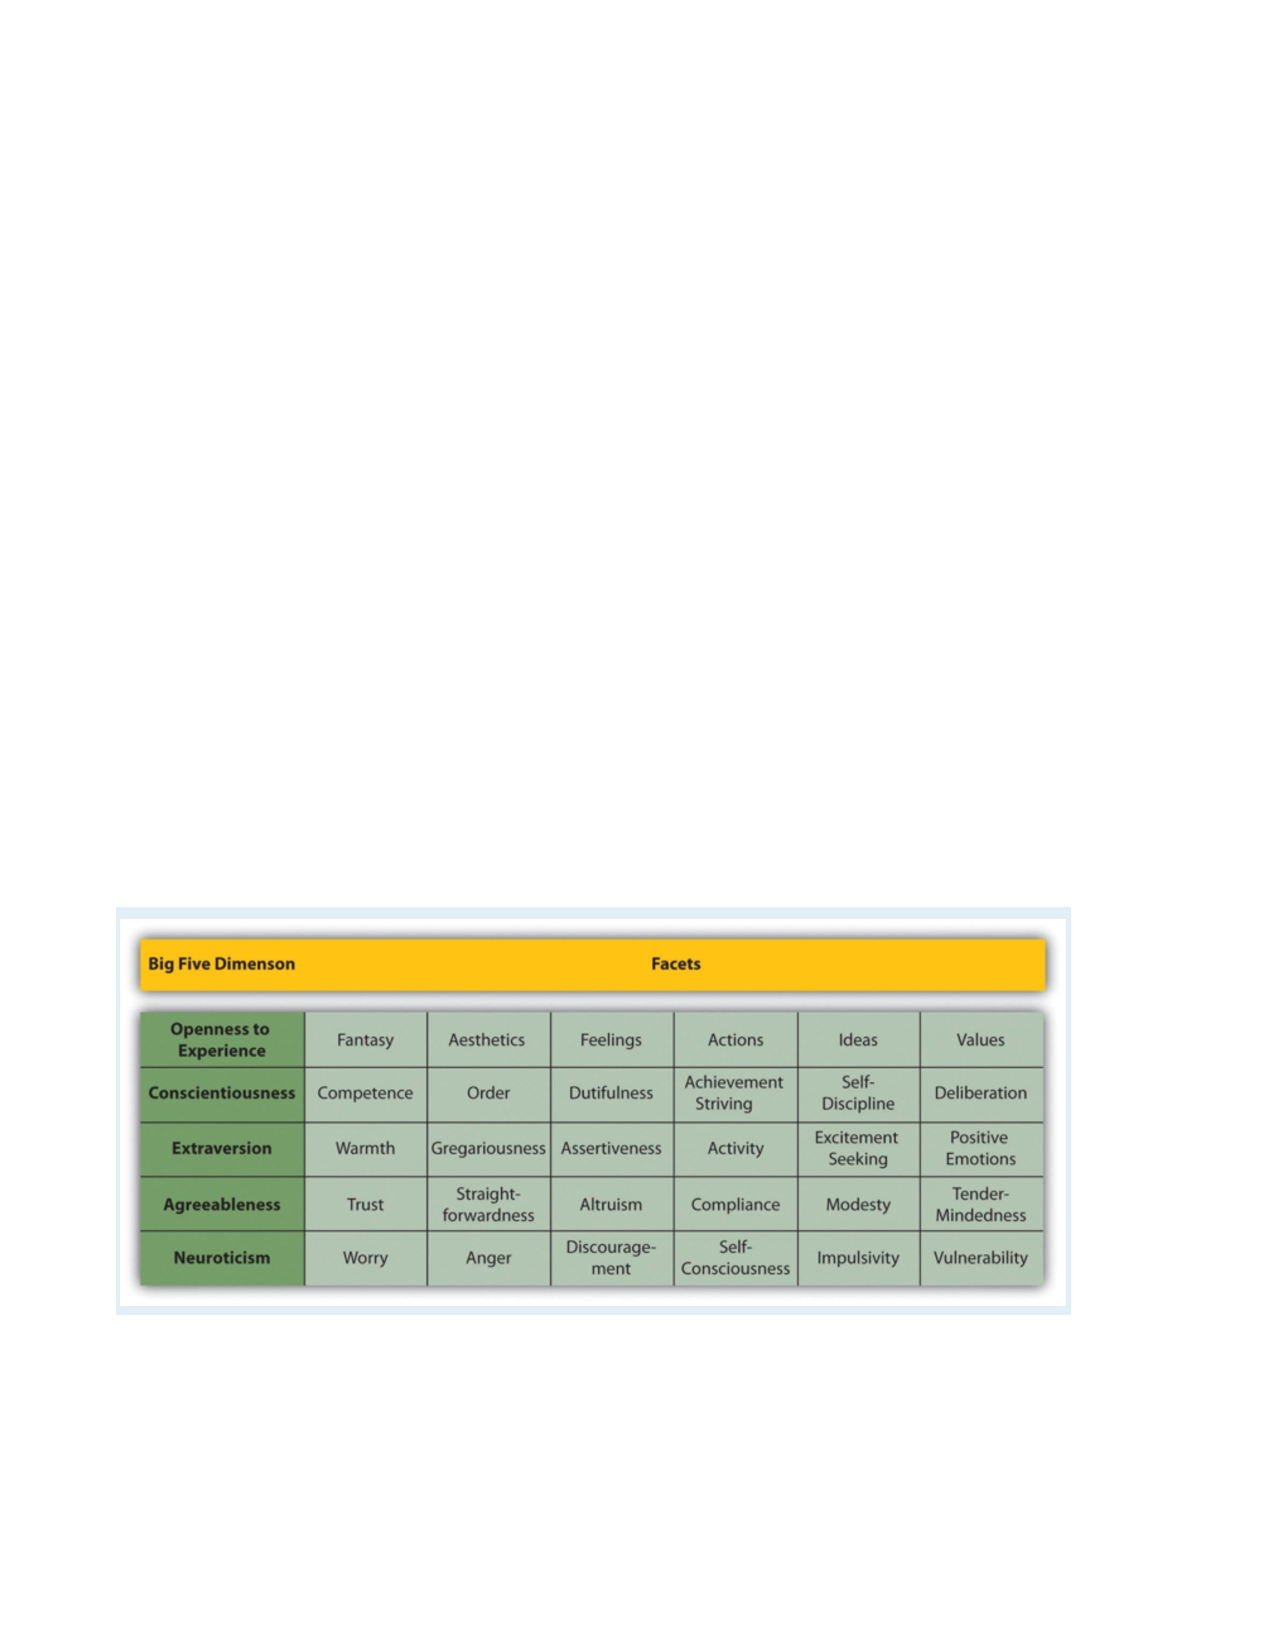
\includegraphics{figures/C5bigfive.pdf}
\caption{The Big Five is a set of five broad dimensions that capture
much of the variation in human personality. Each of the Big Five can
even be defined in terms of six more specific constructs called
``facets'' (Costa \& McCrae, 1992).}
\end{figure}

{[}fig:bigfive{]}

The conceptual definition of a psychological construct describes the
behaviors and internal processes that make up that construct, along with
how it relates to other variables. For example, a conceptual definition
of neuroticism (another one of the Big Five) would be that it is
people's tendency to experience negative emotions such as anxiety,
anger, and sadness across a variety of situations. This definition might
also include that it has a strong genetic component, remains fairly
stable over time, and is positively correlated with the tendency to
experience pain and other physical symptoms.

Students sometimes wonder why, when researchers want to understand a
construct like self-esteem or neuroticism, they do not simply look it up
in the dictionary. One reason is that many scientific constructs do not
have counterparts in everyday language (e.g., working memory capacity).
More important, researchers are in the business of developing
definitions that are more detailed and precise---and that more
accurately describe the way the world is---than the informal definitions
in the dictionary. As we will see, they do this by proposing conceptual
definitions, testing them empirically, and revising them as necessary.
Sometimes they throw them out altogether. This is why the research
literature often includes different conceptual definitions of the same
construct. In some cases, an older conceptual definition has been
replaced by a newer one that fits and works better. In others,
researchers are still in the process of deciding which of various
conceptual definitions is the best.

\section{Operational Definitions}\label{operational-definitions}

An operational definition is a definition of a variable in terms of
precisely how it is to be measured. These measures generally fall into
one of three broad categories. Self-report measures are those in which
participants report on their own thoughts, feelings, and actions, as
with the Rosenberg Self-Esteem Scale. Behavioral measures are those in
which some other aspect of participants' behavior is observed and
recorded. This is an extremely broad category that includes the
observation of people's behavior both in highly structured laboratory
tasks and in more natural settings. A good example of the former would
be measuring working memory capacity using the backward digit span task.
A good example of the latter is a famous operational definition of
physical aggression from researcher Albert Bandura and his colleagues
(Bandura, Ross, \& Ross, 1961)2. They let each of several children play
for 20 minutes in a room that contained a clown-shaped punching bag
called a Bobo doll. They filmed each child and counted the number of
acts of physical aggression he or she committed. These included hitting
the doll with a mallet, punching it, and kicking it. Their operational
definition, then, was the number of these specifically defined acts that
the child committed during the 20-minute period. Finally, physiological
measures are those that involve recording any of a wide variety of
physiological processes, including heart rate and blood pressure,
galvanic skin response, hormone levels, and electrical activity and
blood flow in the brain.

For any given variable or construct, there will be multiple operational
definitions. Stress is a good example. A rough conceptual definition is
that stress is an adaptive response to a perceived danger or threat that
involves physiological, cognitive, affective, and behavioral components.
But researchers have operationally defined it in several ways. The
Social Readjustment Rating Scale is a self-report questionnaire on which
people identify stressful events that they have experienced in the past
year and assigns points for each one depending on its severity. For
example, a man who has been divorced (73 points), changed jobs (36
points), and had a change in sleeping habits (16 points) in the past
year would have a total score of 125. The Daily Hassles and Uplifts
Scale is similar but focuses on everyday stressors like misplacing
things and being concerned about one's weight. The Perceived Stress
Scale is another self-report measure that focuses on people's feelings
of stress (e.g., ``How often have you felt nervous and stressed?'').
Researchers have also operationally defined stress in terms of several
physiological variables including blood pressure and levels of the
stress hormone cortisol.

When psychologists use multiple operational definitions of the same
construct---either within a study or across studies---they are using
converging operations. The idea is that the various operational
definitions are ``converging'' or coming together on the same construct.
When scores based on several different operational definitions are
closely related to each other and produce similar patterns of results,
this constitutes good evidence that the construct is being measured
effectively and that it is useful. The various measures of stress, for
example, are all correlated with each other and have all been shown to
be correlated with other variables such as immune system functioning
(also measured in a variety of ways) (Segerstrom \& Miller, 2004)3. This
is what allows researchers eventually to draw useful general
conclusions, such as ``stress is negatively correlated with immune
system functioning,'' as opposed to more specific and less useful ones,
such as ``people's scores on the Perceived Stress Scale are negatively
correlated with their white blood counts.''

\section{Levels of Measurement}\label{levels-of-measurement}

The psychologist S. S. Stevens suggested that scores can be assigned to
individuals in a way that communicates more or less quantitative
information about the variable of interest (Stevens, 1946). For example,
the officials at a 100-m race could simply rank order the runners as
they crossed the finish line (first, second, etc.), or they could time
each runner to the nearest tenth of a second using a stopwatch (11.5 s,
12.1 s, etc.). In either case, they would be measuring the runners'
times by systematically assigning scores to represent those times. But
while the rank ordering procedure communicates the fact that the
second-place runner took longer to finish than the first- place
finisher, the stopwatch procedure also communicates how much longer the
second-place finisher took. Stevens actually suggested four different
levels of measurement (which he called ``scales of measurement'') that
correspond to four different levels of quantitative information that can
be communicated by a set of scores.

The nominal level of measurement is used for categorical variables and
involves assigning scores that are category labels. Category labels
communicate whether any two individuals are the same or different in
terms of the variable being measured. For example, if you look at your
research participants as they enter the room, decide whether each one is
male or female, and type this information into a spreadsheet, you are
engaged in nominal-level measurement. Or if you ask your participants to
indicate which of several ethnicities they identify themselves with, you
are again engaged in nominal-level measurement. The essential point
about nominal scales is that they do not imply any ordering among the
responses. For example, when classifying people according to their
favorite color, there is no sense in which green is placed ``ahead of''
blue. Responses are merely categorized. Nominal scales thus embody the
lowest level of measurement5.

The remaining three levels of measurement are used for quantitative
variables. The ordinal level of measurement involves assigning scores so
that they represent the rank order of the individuals. Ranks communicate
not only whether any two individuals are the same or different in terms
of the variable being measured but also whether one individual is higher
or lower on that variable. For example, a researcher wishing to measure
consumers' satisfaction with their microwave ovens might ask them to
specify their feelings as either ``very dissatisfied,'' ``somewhat
dissatisfied,'' ``somewhat satisfied,'' or ``very satisfied.'' The items
in this scale are ordered, ranging from least to most satisfied. This is
what distinguishes ordinal from nominal scales. Unlike nominal scales,
ordinal scales allow comparisons of the degree to which two individuals
rate the variable. For example, our satisfaction ordering makes it
meaningful to assert that one person is more satisfied than another with
their microwave ovens. Such an assertion reflects the first person's use
of a verbal label that comes later in the list than the label chosen by
the second person.

On the other hand, ordinal scales fail to capture important information
that will be present in the other levels of measurement we examine. In
particular, the difference between two levels of an ordinal scale cannot
be assumed to be the same as the difference between two other levels
(just like you cannot assume that the gap between the runners in first
and second place is equal to the gap between the runners in second and
third place). In our satisfaction scale, for example, the difference
between the responses ``very dissatisfied'' and ``somewhat
dissatisfied'' is probably not equivalent to the difference between
``somewhat dissatisfied'' and ``somewhat satisfied.'' Nothing in our
measurement procedure allows us to determine whether the two differences
reflect the same difference in psychological satisfaction. Statisticians
express this point by saying that the differences between adjacent scale
values do not necessarily represent equal intervals on the underlying
scale giving rise to the measurements. (In our case, the underlying
scale is the true feeling of satisfaction, which we are trying to
measure.)

The interval level of measurement involves assigning scores using
numerical scales in which intervals have the same interpretation
throughout. As an example, consider either the Fahrenheit or Celsius
temperature scales. The difference between 30 degrees and 40 degrees
represents the same temperature difference as the difference between 80
degrees and 90 degrees. This is because each 10-degree interval has the
same physical meaning (in terms of the kinetic energy of molecules).

Interval scales are not perfect, however. In particular, they do not
have a true zero point even if one of the scaled values happens to carry
the name ``zero.'' The Fahrenheit scale illustrates the issue. Zero
degrees Fahrenheit does not represent the complete absence of
temperature (the absence of any molecular kinetic energy). In reality,
the label ``zero'' is applied to its temperature for quite accidental
reasons connected to the history of temperature measurement. Since an
interval scale has no true zero point, it does not make sense to compute
ratios of temperatures. For example, there is no sense in which the
ratio of 40 to 20 degrees Fahrenheit is the same as the ratio of 100 to
50 degrees; no interesting physical property is preserved across the two
ratios. After all, if the ``zero'' label were applied at the temperature
that Fahrenheit happens to label as 10 degrees, the two ratios would
instead be 30 to 10 and 90 to 40, no longer the same! For this reason,
it does not make sense to say that 80 degrees is ``twice as hot'' as 40
degrees. Such a claim would depend on an arbitrary decision about where
to ``start'' the temperature scale, namely, what temperature to call
zero (whereas the claim is intended to make a more fundamental assertion
about the underlying physical reality). In psychology, the intelligence
quotient (IQ) is often considered to be measured at the interval level.

Finally, the ratio level of measurement involves assigning scores in
such a way that there is a true zero point that represents the complete
absence of the quantity. Height measured in meters and weight measured
in kilograms are good examples. So are counts of discrete objects or
events such as the number of siblings one has or the number of questions
a student answers correctly on an exam. You can think of a ratio scale
as the three earlier scales rolled up in one. Like a nominal scale, it
provides a name or category for each object (the numbers serve as
labels). Like an ordinal scale, the objects are ordered (in terms of the
ordering of the numbers). Like an interval scale, the same difference at
two places on the scale has the same meaning. However, in addition, the
same ratio at two places on the scale also carries the same meaning (see
Table 5.1).

The Fahrenheit scale for temperature has an arbitrary zero point and is
therefore not a ratio scale. However, zero on the Kelvin scale is
absolute zero. This makes the Kelvin scale a ratio scale. For example,
if one temperature is twice as high as another as measured on the Kelvin
scale, then it has twice the kinetic energy of the other temperature.

Another example of a ratio scale is the amount of money you have in your
pocket right now (25 cents, 50 cents, etc.). Money is measured on a
ratio scale because, in addition to having the properties of an interval
scale, it has a true zero point: if you have zero money, this actually
implies the absence of money. Since money has a true zero point, it
makes sense to say that someone with 50 cents has twice as much money as
someone with 25 cents.

\begin{figure}[htbp]
\centering
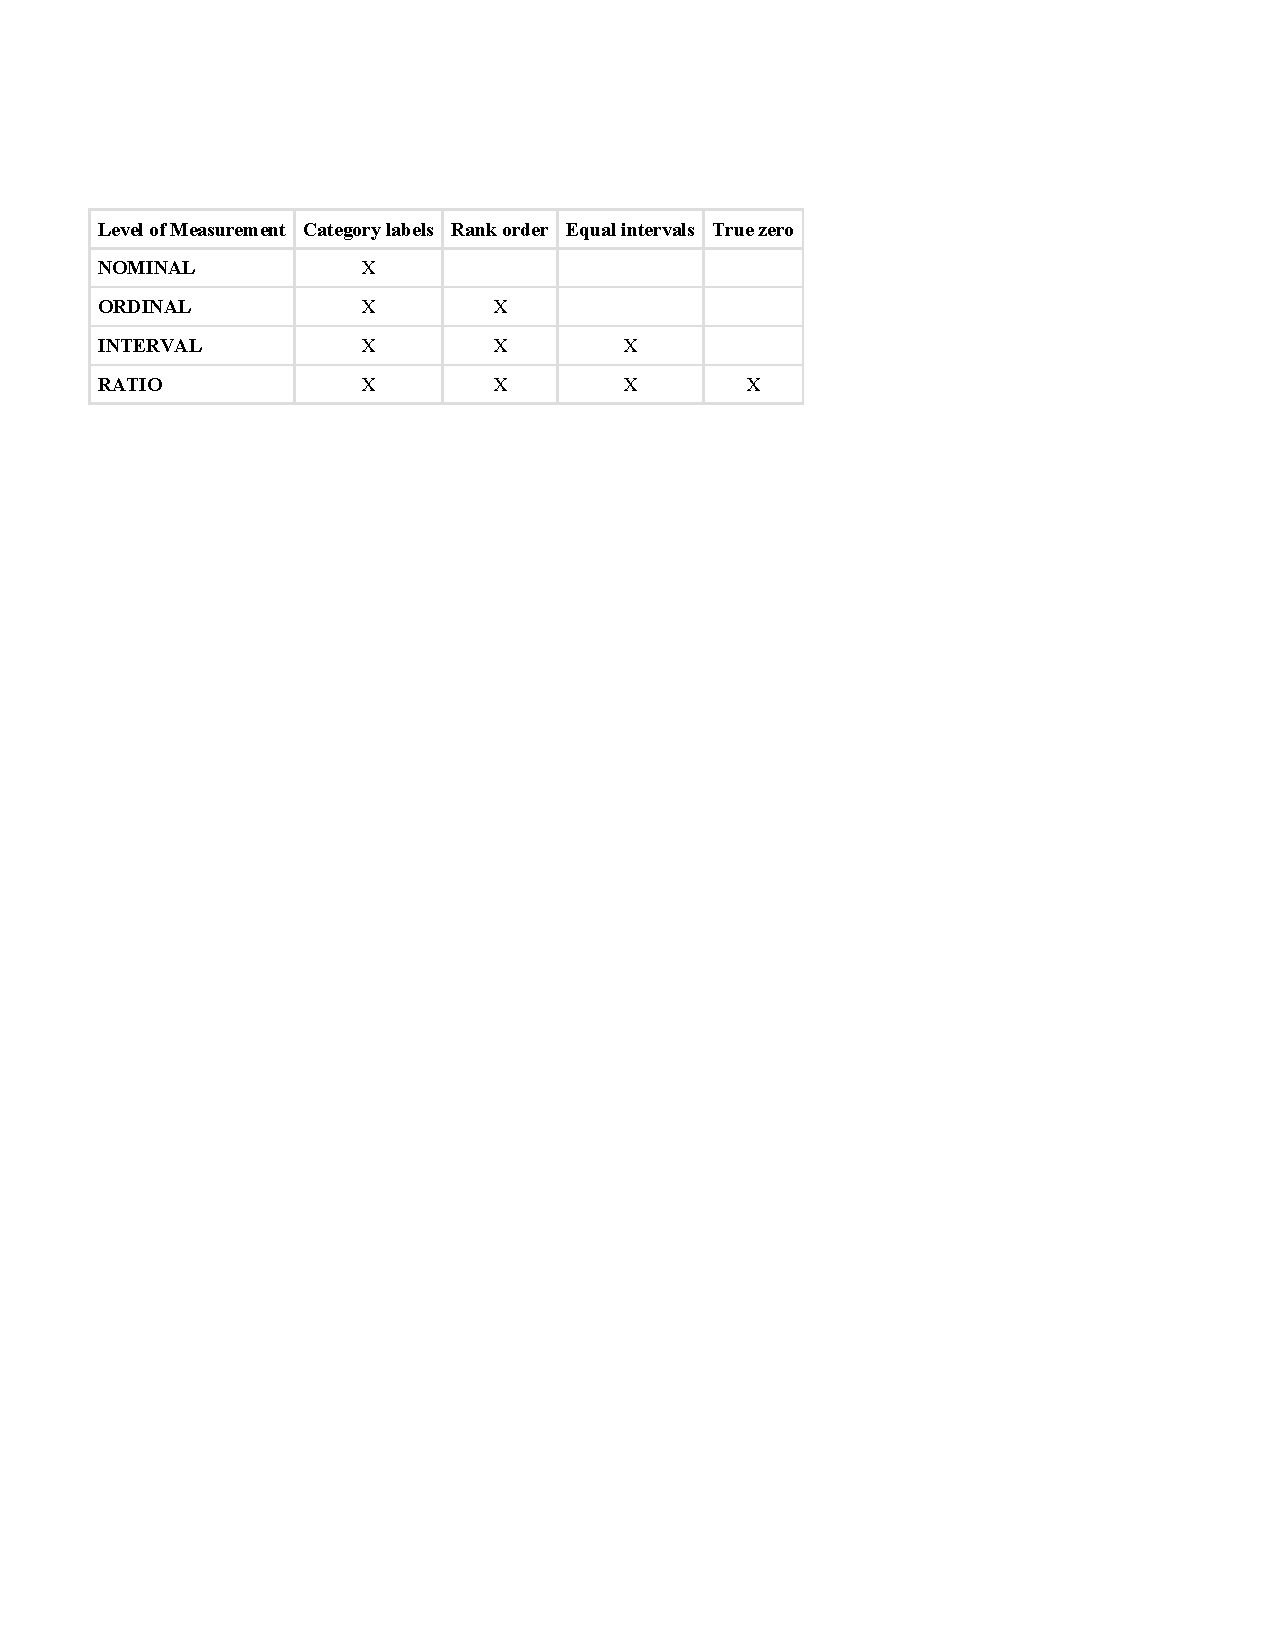
\includegraphics{figures/C5Mscales.pdf}
\caption{Summary of levels of measurement}
\end{figure}

{[}fig:scales{]}

Stevens's levels of measurement are important for at least two reasons.
First, they emphasize the generality of the concept of measurement.
Although people do not normally think of categorizing or ranking
individuals as measurement, in fact they are as long as they are done so
that they represent some characteristic of the individuals. Second, the
levels of measurement can serve as a rough guide to the statistical
procedures that can be used with the data and the conclusions that can
be drawn from them. With nominal-level measurement, for example, the
only available measure of central tendency is the mode. Also,
ratio-level measurement is the only level that allows meaningful
statements about ratios of scores. One cannot say that someone with an
IQ of 140 is twice as intelligent as someone with an IQ of 70 because IQ
is measured at the interval level, but one can say that someone with six
siblings has twice as many as someone with three because number of
siblings is measured at the ratio level.

\begin{itemize}
\item
  Measurement is the assignment of scores to individuals so that the
  scores represent some characteristic of the individuals. Psychological
  measurement can be achieved in a wide variety of ways, including
  self-report, behavioral, and physiological measures.
\item
  Psychological constructs such as intelligence, self-esteem, and
  depression are variables that are not directly observable because they
  represent behavioral tendencies or complex patterns of behavior and
  internal processes. An important goal of scientific research is to
  conceptually define psychological constructs in ways that accurately
  describe them.
\item
  For any conceptual definition of a construct, there will be many
  different operational definitions or ways of measuring it. The use of
  multiple operational definitions, or converging operations, is a
  common strategy in psychological research.
\item
  Variables can be measured at four different levels---nominal, ordinal,
  interval, and ratio---that communicate increasing amounts of
  quantitative information. The level of measurement affects the kinds
  of statistics you can use and conclusions you can draw from your data.
\end{itemize}

\begin{enumerate}
\def\labelenumi{\arabic{enumi}.}
\item
  Practice: Complete the Rosenberg Self-Esteem Scale and compute your
  overall score.
\item
  Practice: Think of three operational definitions for sexual jealousy,
  decisiveness, and social anxiety. Consider the possibility of
  self-report, behavioral, and physiological measures. Be as precise as
  you can.
\item
  Practice: For each of the following variables, decide which level of
  measurement is being used.

  \begin{itemize}
  \item
    An university instructor measures the time it takes her students to
    finish an exam by looking through the stack of exams at the end. She
    assigns the one on the bottom a score of 1, the one on top of that a
    2, and so on.
  \item
    A researcher accesses her participants' medical records and counts
    the number of times they have seen a doctor in the last year
  \item
    Participants in a study are asked whether they are right or left
    handed
  \end{itemize}
\end{enumerate}

\chapter{Reliability and Validity of
Measurement}\label{reliability-and-validity-of-measurement}

Again, measurement involves assigning scores to individuals so that they
represent some characteristic of the individuals. But how do researchers
know that the scores actually represent the characteristic, especially
when it is a construct like intelligence, self-esteem, depression, or
working memory capacity? The answer is that they conduct research using
the measure to confirm that the scores make sense based on their
understanding of the construct being measured. This is an extremely
important point. Psychologists do not simply assume that their measures
work. Instead, they collect data to demonstrate that they work. If their
research does not demonstrate that a measure works, they stop using it.

As an informal example, imagine that you have been dieting for a month.
Your clothes seem to be fitting more loosely, and several friends have
asked if you have lost weight. If at this point your bathroom scale
indicated that you had lost 10 pounds, this would make sense and you
would continue to use the scale. But if it indicated that you had gained
10 pounds, you would rightly conclude that it was broken and either fix
it or get rid of it. In evaluating a measurement method, psychologists
consider two general dimensions: reliability and validity. We will go
into these two dimensions in depth in the next sections. In general,
reliability is about whether the measurement is free from error, and
behaves consistently. Validity is about what the measure means (does
your measure actually measure what you want it to).

\section{Reliability}\label{reliability}

Reliability refers to the consistency of a measure. Psychologists
consider three types of consistency: over time (test- retest
reliability), across items (internal consistency), and across different
researchers (inter-rater reliability).

\section{Test-Retest Reliability}\label{test-retest-reliability}

When researchers measure a construct that they assume to be consistent
across time, then the scores they obtain should also be consistent
across time. Test-retest reliability is the extent to which this is
actually the case. For example, intelligence is generally thought to be
consistent across time. A person who is highly intelligent today will be
highly intelligent next week. This means that any good measure of
intelligence should produce roughly the same scores for this individual
next week as it does today. Clearly, a measure that produces highly
inconsistent scores over time cannot be a very good measure of a
construct that is supposed to be consistent.

Assessing test-retest reliability requires using the measure on a group
of people at one time, using it again on the same group of people at a
later time, and then looking at test-retest correlation between the two
sets of scores. This is typically done by graphing the data in a
scatterplot and computing Pearson's r. Figure 5.2 shows the correlation
between two sets of scores of several university students on the
Rosenberg Self-Esteem Scale, administered two times, a week apart.
Pearson's r for these data is +.95. In general, a test-retest
correlation of +.80 or greater is considered to indicate good
reliability.

\begin{figure}[htbp]
\centering
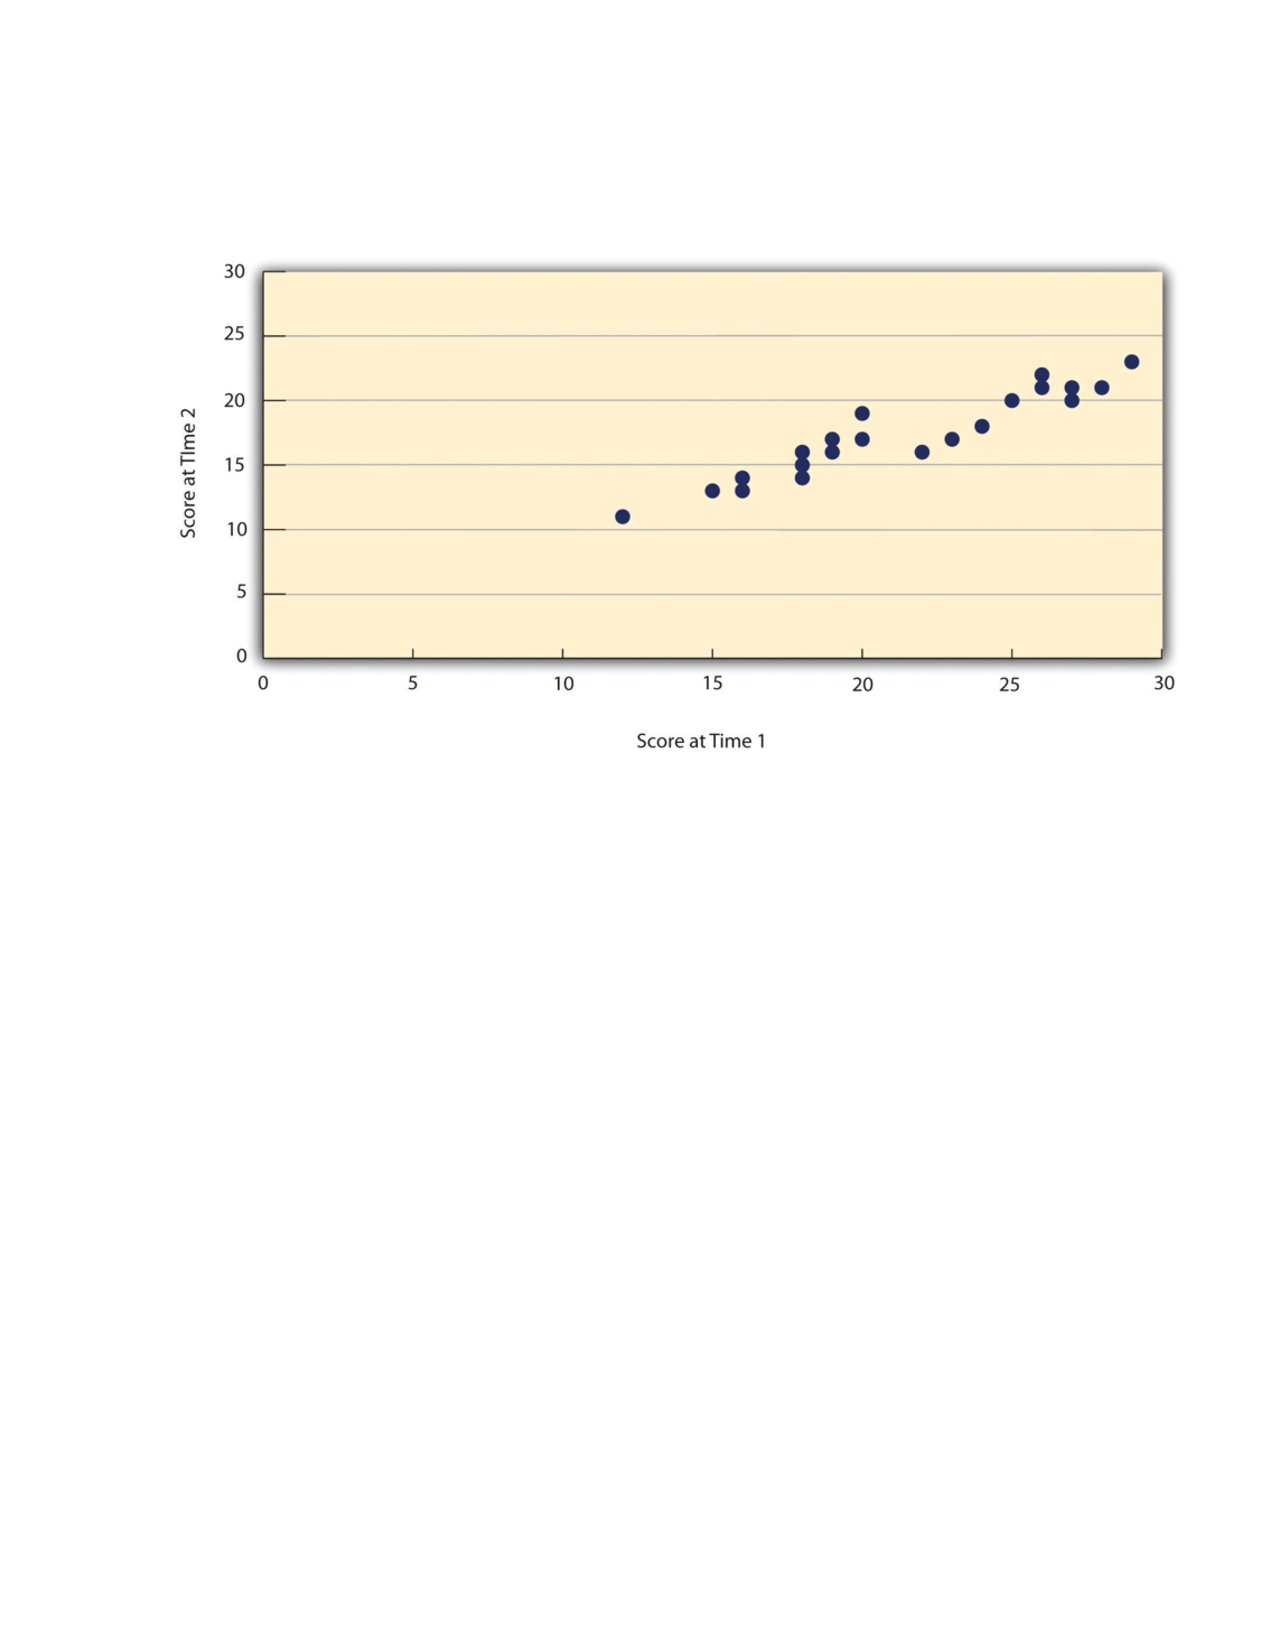
\includegraphics{figures/C5testretest.pdf}
\caption{Test-Retest Correlation Between Two Sets of Scores of Several
College Students on the Rosenberg Self-Esteem Scale, Given Two Times a
Week Apart}
\end{figure}

{[}fig:testretest{]}

Again, high test-retest correlations make sense when the construct being
measured is assumed to be consistent over time, which is the case for
intelligence, self-esteem, and the Big Five personality dimensions. But
other constructs are not assumed to be stable over time. The very nature
of mood, for example, is that it changes. So a measure of mood that
produced a low test-retest correlation over a period of a month would
not be a cause for concern.

\section{Internal Consistency}\label{internal-consistency}

A second kind of reliability is internal consistency, which is the
consistency of people's responses across the items on a multiple-item
measure. In general, all the items on such measures are supposed to
reflect the same underlying construct, so people's scores on those items
should be correlated with each other. On the Rosenberg Self-Esteem
Scale, people who agree that they are a person of worth should tend to
agree that that they have a number of good qualities. If people's
responses to the different items are not correlated with each other,
then it would no longer make sense to claim that they are all measuring
the same underlying construct. This is as true for behavioral and
physiological measures as for self-report measures. For example, people
might make a series of bets in a simulated game of roulette as a measure
of their level of risk seeking. This measure would be internally
consistent to the extent that individual participants' bets were
consistently high or low across trials.

Like test-retest reliability, internal consistency can only be assessed
by collecting and analyzing data. One approach is to look at a
split-half correlation. This involves splitting the items into two sets,
such as the first and second halves of the items or the even- and
odd-numbered items. Then a score is computed for each set of items, and
the relationship between the two sets of scores is examined. For
example, Figure 5.3 shows the split-half correlation between several
university students' scores on the even-numbered items and their scores
on the odd-numbered items of the Rosenberg Self-Esteem Scale. Pearson's
r for these data is +.88. A split-half correlation of +.80 or greater is
generally considered good internal consistency.

\begin{figure}[htbp]
\centering
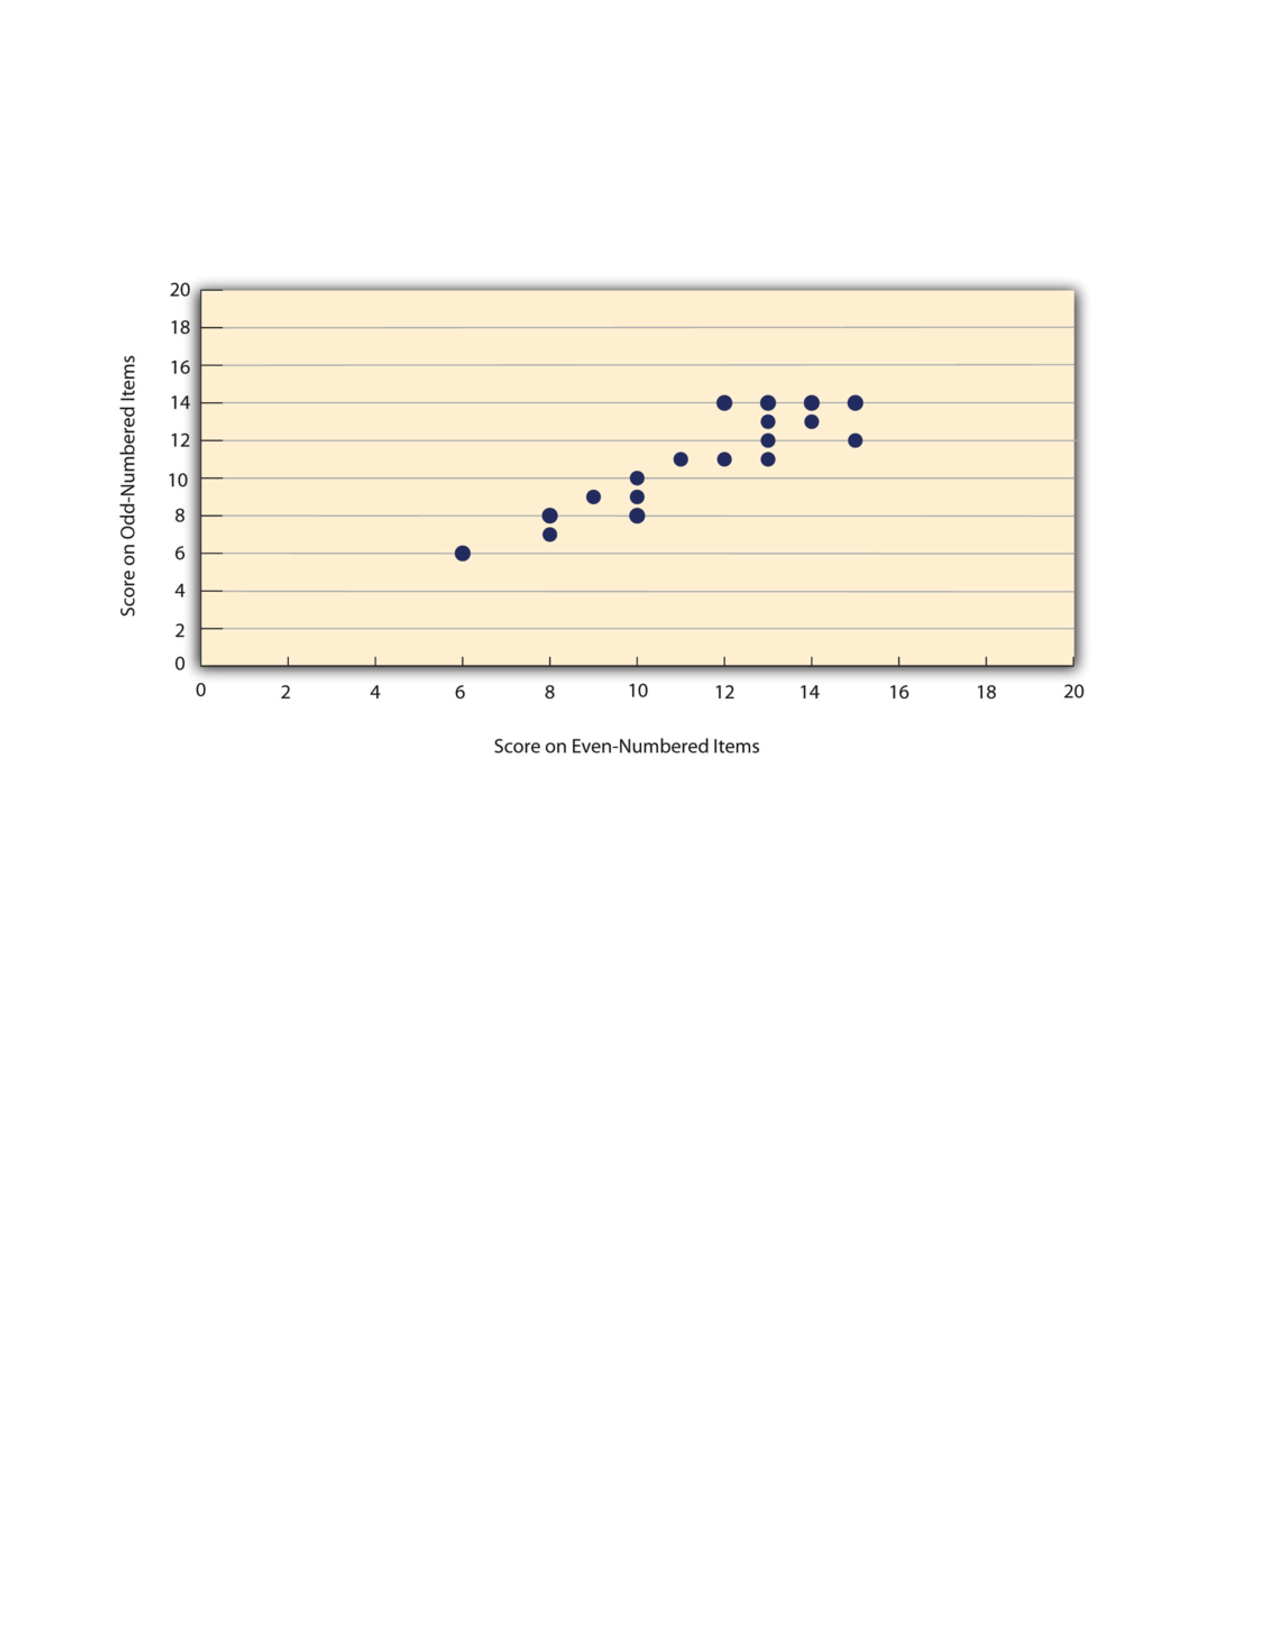
\includegraphics{figures/C5internal.pdf}
\caption{Split-Half Correlation Between Several College Students' Scores
on the Even-Numbered Items and Their Scores on the Odd-Numbered Items of
the Rosenberg Self-Esteem Scale}
\end{figure}

{[}fig:testretest{]}

Perhaps the most common measure of internal consistency used by
researchers in psychology is a statistic called Cronbach's \(\alpha\)
(the Greek letter alpha). Conceptually, \(\alpha\) is the mean of all
possible split-half correlations for a set of items. For example, there
are 252 ways to split a set of 10 items into two sets of five.
Cronbach's \(\alpha\) would be the mean of the 252 split-half
correlations. Note that this is not how \(\alpha\) is actually computed,
but it is a correct way of interpreting the meaning of this statistic.
Again, a value of +.80 or greater is generally taken to indicate good
internal consistency.

\section{Inter-rater Reliability}\label{inter-rater-reliability}

Many behavioral measures involve significant judgment on the part of an
observer or a rater.Inter- rater reliability is the extent to which
different observers are consistent in their judgments. For example, if
you were interested in measuring university students' social skills, you
could make video recordings of them as they interacted with another
student whom they are meeting for the first time. Then you could have
two or more observers watch the videos and rate each student's level of
social skills. To the extent that each participant does in fact have
some level of social skills that can be detected by an attentive
observer, different observers' ratings should be highly correlated with
each other. Inter-rater reliability would also have been measured in
Bandura's Bobo doll study. In this case, the observers' ratings of how
many acts of aggression a particular child committed while playing with
the Bobo doll should have been highly positively correlated. Interrater
reliability is often assessed using Cronbach's \(\alpha\) when the
judgments are quantitative or an analogous statistic called Cohen's
\(\kappa\) (the Greek letter kappa) when they are categorical.

\section{Validity}\label{validity}

Validity is the extent to which the scores from a measure represent the
variable they are intended to. But how do researchers make this
judgment? We have already considered one factor that they take into
account---reliability. When a measure has good test-retest reliability
and internal consistency, researchers should be more confident that the
scores represent what they are supposed to. There has to be more to it,
however, because a measure can be extremely reliable but have no
validity whatsoever. As an absurd example, imagine someone who believes
that people's index finger length reflects their self-esteem and
therefore tries to measure self-esteem by holding a ruler up to people's
index fingers. Although this measure would have extremely good
test-retest reliability, it would have absolutely no validity. The fact
that one person's index finger is a centimeter longer than another's
would indicate nothing about which one had higher self-esteem.

Discussions of validity usually divide it into several distinct
``types.'' But a good way to interpret these types is that they are
other kinds of evidence---in addition to reliability---that should be
taken into account when judging the validity of a measure. Here we
consider three basic kinds: face validity, content validity, and
criterion validity.

\section{Face Validity}\label{face-validity}

Face validity is the extent to which a measurement method appears ``on
its face'' to measure the construct of interest. Most people would
expect a self-esteem questionnaire to include items about whether they
see themselves as a person of worth and whether they think they have
good qualities. So a questionnaire that included these kinds of items
would have good face validity. The finger-length method of measuring
self-esteem, on the other hand, seems to have nothing to do with
self-esteem and therefore has poor face validity. Although face validity
can be assessed quantitatively---for example, by having a large sample
of people rate a measure in terms of whether it appears to measure what
it is intended to---it is usually assessed informally.

Face validity is at best a very weak kind of evidence that a measurement
method is measuring what it is supposed to. One reason is that it is
based on people's intuitions about human behavior, which are frequently
wrong. It is also the case that many established measures in psychology
work quite well despite lacking face validity. The Minnesota Multiphasic
Personality Inventory-2 (MMPI-2) measures many personality
characteristics and disorders by having people decide whether each of
over 567 different statements applies to them---where many of the
statements do not have any obvious relationship to the construct that
they measure. For example, the items ``I enjoy detective or mystery
stories'' and ``The sight of blood doesn't frighten me or make me sick''
both measure the suppression of aggression. In this case, it is not the
participants' literal answers to these questions that are of interest,
but rather whether the pattern of the participants' responses to a
series of questions matches those of individuals who tend to suppress
their aggression.

\section{Content Validity}\label{content-validity}

Content validity is the extent to which a measure ``covers'' the
construct of interest. For example, if a researcher conceptually defines
test anxiety as involving both sympathetic nervous system activation
(leading to nervous feelings) and negative thoughts, then his measure of
test anxiety should include items about both nervous feelings and
negative thoughts. Or consider that attitudes are usually defined as
involving thoughts, feelings, and actions toward something. By this
conceptual definition, a person has a positive attitude toward exercise
to the extent that he or she thinks positive thoughts about exercising,
feels good about exercising, and actually exercises. So to have good
content validity, a measure of people's attitudes toward exercise would
have to reflect all three of these aspects. Like face validity, content
validity is not usually assessed quantitatively. Instead, it is assessed
by carefully checking the measurement method against the conceptual
definition of the construct.

\section{Criterion Validity}\label{criterion-validity}

Criterion validity is the extent to which people's scores on a measure
are correlated with other variables (known as criteria) that one would
expect them to be correlated with. For example, people's scores on a new
measure of test anxiety should be negatively correlated with their
performance on an important school exam. If it were found that people's
scores were in fact negatively correlated with their exam performance,
then this would be a piece of evidence that these scores really
represent people's test anxiety. But if it were found that people scored
equally well on the exam regardless of their test anxiety scores, then
this would cast doubt on the validity of the measure.

A criterion can be any variable that one has reason to think should be
correlated with the construct being measured, and there will usually be
many of them. For example, one would expect test anxiety scores to be
negatively correlated with exam performance and course grades and
positively correlated with general anxiety and with blood pressure
during an exam. Or imagine that a researcher develops a new measure of
physical risk taking. People's scores on this measure should be
correlated with their participation in ``extreme'' activities such as
snowboarding and rock climbing, the number of speeding tickets they have
received, and even the number of broken bones they have had over the
years. When the criterion is measured at the same time as the construct,
criterion validity is referred to as concurrent validity; however, when
the criterion is measured at some point in the future (after the
construct has been measured), it is referred to as predictive validity
(because scores on the measure have ``predicted'' a future outcome).

Criteria can also include other measures of the same construct. For
example, one would expect new measures of test anxiety or physical risk
taking to be positively correlated with existing measures of the same
constructs. This is known as convergent validity.

Assessing convergent validity requires collecting data using the
measure. Researchers John Cacioppo and Richard Petty did this when they
created their self-report Need for Cognition Scale to measure how much
people value and engage in thinking (Cacioppo \& Petty, 1982). In a
series of studies, they showed that people's scores were positively
correlated with their scores on a standardized academic achievement
test, and that their scores were negatively correlated with their scores
on a measure of dogmatism (which represents a tendency toward
obedience). In the years since it was created, the Need for Cognition
Scale has been used in literally hundreds of studies and has been shown
to be correlated with a wide variety of other variables, including the
effectiveness of an advertisement, interest in politics, and juror
decisions (Petty, Briñol, Loersch, \& McCaslin, 2009).

\section{Discriminant Validity}\label{discriminant-validity}

Discriminant validity, on the other hand, is the extent to which scores
on a measure are not correlated with measures of variables that are
conceptually distinct. For example, self-esteem is a general attitude
toward the self that is fairly stable over time. It is not the same as
mood, which is how good or bad one happens to be feeling right now. So
people's scores on a new measure of self-esteem should not be very
highly correlated with their moods. If the new measure of self-esteem
were highly correlated with a measure of mood, it could be argued that
the new measure is not really measuring self-esteem; it is measuring
mood instead.

When they created the Need for Cognition Scale, Cacioppo and Petty also
provided evidence of discriminant validity by showing that people's
scores were not correlated with certain other variables. For example,
they found only a weak correlation between people's need for cognition
and a measure of their cognitive style---the extent to which they tend
to think analytically by breaking ideas into smaller parts or
holistically in terms of ``the big picture.'' They also found no
correlation between people's need for cognition and measures of their
test anxiety and their tendency to respond in socially desirable ways.
All these low correlations provide evidence that the measure is
reflecting a conceptually distinct construct.

\begin{itemize}
\item
  Psychological researchers do not simply assume that their measures
  work. Instead, they conduct research to show that they work. If they
  cannot show that they work, they stop using them.
\item
  There are two distinct criteria by which researchers evaluate their
  measures: reliability and validity. Reliability is consistency across
  time (test-retest reliability), across items (internal consistency),
  and across researchers (interrater reliability). Validity is the
  extent to which the scores actually represent the variable they are
  intended to.
\item
  Validity is a judgment based on various types of evidence. The
  relevant evidence includes the measure's reliability, whether it
  covers the construct of interest, and whether the scores it produces
  are correlated with other variables they are expected to be correlated
  with and not correlated with variables that are conceptually distinct.
\item
  The reliability and validity of a measure is not established by any
  single study but by the pattern of results across multiple studies.
  The assessment of reliability and validity is an ongoing process.
\end{itemize}

\begin{enumerate}
\def\labelenumi{\arabic{enumi}.}
\item
  Practice: Ask several friends to complete the Rosenberg Self-Esteem
  Scale. Then assess its internal consistency by making a scatterplot to
  show the split-half correlation (even- vs.~odd- numbered items).
  Compute Pearson's r too if you know how.
\item
  Think back to the last college exam you took and think of the exam as
  a psychological measure. What construct do you think it was intended
  to measure? Comment on its face and content validity. What data could
  you collect to assess its reliability and criterion validity?
\end{enumerate}

\chapter{Practical Strategies for Psychological
Measurement}\label{practical-strategies-for-psychological-measurement}

So far in this chapter, we have considered several basic ideas about the
nature of psychological constructs and their measurement. But now
imagine that you are in the position of actually having to measure a
psychological construct for a research project. How should you proceed?
Broadly speaking, there are four steps in the measurement process: (a)
conceptually defining the construct, (b) operationally defining the
construct, (c) implementing the measure, and (d) evaluating the measure.
In this section, we will look at each of these steps in turn.

\section{Conceptually Defining the
Construct}\label{conceptually-defining-the-construct}

Having a clear and complete conceptual definition of a construct is a
prerequisite for good measurement. For one thing, it allows you to make
sound decisions about exactly how to measure the construct. If you had
only a vague idea that you wanted to measure people's ``memory,'' for
example, you would have no way to choose whether you should have them
remember a list of vocabulary words, a set of photographs, a newly
learned skill, or an experience from long ago. Because psychologists now
conceptualize memory as a set of semi-independent systems, you would
have to be more precise about what you mean by ``memory.'' If you are
interested in long-term semantic memory (memory for facts), then having
participants remember a list of words that they learned last week would
make sense, but having them remember and execute a newly learned skill
would not. In general, there is no substitute for reading the research
literature on a construct and paying close attention to how others have
defined it.

\section{Deciding on an Operational
Definition}\label{deciding-on-an-operational-definition}

\section{Using an Existing Measure}\label{using-an-existing-measure}

It is usually a good idea to use an existing measure that has been used
successfully in previous research. Among the advantages are that (a) you
save the time and trouble of creating your own, (b) there is already
some evidence that the measure is valid (if it has been used
successfully), and (c) your results can more easily be compared with and
combined with previous results. In fact, if there already exists a
reliable and valid measure of a construct, other researchers might
expect you to use it unless you have a good and clearly stated reason
for not doing so.

If you choose to use an existing measure, you may still have to choose
among several alternatives. You might choose the most common one, the
one with the best evidence of reliability and validity, the one that
best measures a particular aspect of a construct that you are interested
in (e.g., a physiological measure of stress if you are most interested
in its underlying physiology), or even the one that would be easiest to
use. For example, the Ten-Item Personality Inventory (TIPI) is a
self-report questionnaire that measures all the Big Five personality
dimensions with just 10 items (Gosling, Rentfrow, \& Swann, 2003)1. It
is not as reliable or valid as longer and more comprehensive measures,
but a researcher might choose to use it when testing time is severely
limited.

When an existing measure was created primarily for use in scientific
research, it is usually described in detail in a published research
article and is free to use in your own research---with a proper
citation. You might find that later researchers who use the same measure
describe it only briefly but provide a reference to the original
article, in which case you would have to get the details from the
original article. The American Psychological Association also publishes
the Directory of Unpublished Experimental Measures, which is an
extensive catalog of measures that have been used in previous research.
Many existing measures---especially those that have applications in
clinical psychology---are proprietary. This means that a publisher owns
the rights to them and that you would have to purchase them. These
include many standard intelligence tests, the Beck Depression Inventory,
and the Minnesota Multiphasic Personality Inventory (MMPI). Details
about many of these measures and how to obtain them can be found in
other reference books, including Tests in Print and the Mental
Measurements Yearbook. There is a good chance you can find these
reference books in your university library.

\section{Creating Your Own Measure}\label{creating-your-own-measure}

Instead of using an existing measure, you might want to create your own.
Perhaps there is no existing measure of the construct you are interested
in or existing ones are too difficult or time-consuming to use. Or
perhaps you want to use a new measure specifically to see whether it
works in the same way as existing measures---that is, to evaluate
convergent validity. In this section, we consider some general issues in
creating new measures that apply equally to self-report, behavioral, and
physiological measures. More detailed guidelines for creating
self-report measures are presented in Chapter 9.

First, be aware that most new measures in psychology are really
variations of existing measures, so you should still look to the
research literature for ideas. Perhaps you can modify an existing
questionnaire, create a paper-and- pencil version of a measure that is
normally computerized (or vice versa), or adapt a measure that has
traditionally been used for another purpose. For example, the famous
Stroop task (Stroop, 1935)2---in which people quickly name the colors
that various color words are printed in---has been adapted for the study
of social anxiety. Socially anxious people are slower at color naming
when the words have negative social connotations such as ``stupid''
(Amir, Freshman, \& Foa, 2002)3.

When you create a new measure, you should strive for simplicity.
Remember that your participants are not as interested in your research
as you are and that they will vary widely in their ability to understand
and carry out whatever task you give them. You should create a set of
clear instructions using simple language that you can present in writing
or read aloud (or both). It is also a good idea to include one or more
practice items so that participants can become familiar with the task,
and to build in an opportunity for them to ask questions before
continuing. It is also best to keep the measure brief to avoid boring or
frustrating your participants to the point that their responses start to
become less reliable and valid.

The need for brevity, however, needs to be weighed against the fact that
it is nearly always better for a measure to include multiple items
rather than a single item. There are two reasons for this. One is a
matter of content validity. Multiple items are often required to cover a
construct adequately. The other is a matter of reliability. People's
responses to single items can be influenced by all sorts of irrelevant
factors---misunderstanding the particular item, a momentary distraction,
or a simple error such as checking the wrong response option. But when
several responses are summed or averaged, the effects of these
irrelevant factors tend to cancel each other out to produce more
reliable scores. Remember, however, that multiple items must be
structured in a way that allows them to be combined into a single
overall score by summing or averaging. To measure ``financial
responsibility,'' a student might ask people about their annual income,
obtain their credit score, and have them rate how ``thrifty'' they
are---but there is no obvious way to combine these responses into an
overall score. To create a true multiple-item measure, the student might
instead ask people to rate the degree to which 10 statements about
financial responsibility describe them on the same five-point scale.

Finally, the very best way to assure yourself that your measure has
clear instructions, includes sufficient practice, and is an appropriate
length is to test several people. (Family and friends often serve this
purpose nicely). Observe them as they complete the task, time them, and
ask them afterward to comment on how easy or difficult it was, whether
the instructions were clear, and anything else you might be wondering
about. Obviously, it is better to discover problems with a measure
before beginning any large-scale data collection.

\section{Implementing the Measure}\label{implementing-the-measure}

You will want to implement any measure in a way that maximizes its
reliability and validity. In most cases, it is best to test everyone
under similar conditions that, ideally, are quiet and free of
distractions. Testing participants in groups is often done because it is
efficient, but be aware that it can create distractions that reduce the
reliability and validity of the measure. As always, it is good to use
previous research as a guide. If others have successfully tested people
in groups using a particular measure, then you should consider doing it
too.

Be aware also that people can react in a variety of ways to being
measured that reduce the reliability and validity of the scores.
Although some disagreeable participants might intentionally respond in
ways meant to disrupt a study, participant reactivity is more likely to
take the opposite form. Agreeable participants might respond in ways
they believe they are expected to. They might engage in socially
desirable responding. For example, people with low self-esteem agree
that they feel they are a person of worth not because they really feel
this way but because they believe this is the socially appropriate
response and do not want to look bad in the eyes of the researcher.
Additionally, research studies can have built-in demand characteristics:
subtle cues that reveal how the researcher expects participants to
behave. For example, a participant whose attitude toward exercise is
measured immediately after she is asked to read a passage about the
dangers of heart disease might reasonably conclude that the passage was
meant to improve her attitude. As a result, she might respond more
favorably because she believes she is expected to by the researcher.
Finally, your own expectations can bias participants' behaviors in
unintended ways.

There are several precautions you can take to minimize these kinds of
reactivity. One is to make the procedure as clear and brief as possible
so that participants are not tempted to vent their frustrations on your
results. Another is to guarantee participants' anonymity and make clear
to them that you are doing so. If you are testing them in groups, be
sure that they are seated far enough apart that they cannot see each
other's responses. Give them all the same type of writing implement so
that they cannot be identified by, for example, the pink glitter pen
that they used. You can even allow them to seal completed questionnaires
into individual envelopes or put them into a drop box where they
immediately become mixed with others' questionnaires. Although informed
consent requires telling participants what they will be doing, it does
not require revealing your hypothesis or other information that might
suggest to participants how you expect them to respond. A questionnaire
designed to measure financial responsibility need not be titled ``Are
You Financially Responsible?'' It could be titled ``Money
Questionnaire'' or have no title at all. Finally, the effects of your
expectations can be minimized by arranging to have the measure
administered by a helper who is ``blind'' or unaware of its intent or of
any hypothesis being tested. Regardless of whether this is possible, you
should standardize all interactions between researchers and
participants---for example, by always reading the same set of
instructions word for word.

\section{Evaluating the Measure}\label{evaluating-the-measure}

Once you have used your measure on a sample of people and have a set of
scores, you are in a position to evaluate it more thoroughly in terms of
reliability and validity. Even if the measure has been used extensively
by other researchers and has already shown evidence of reliability and
validity, you should not assume that it worked as expected for your
particular sample and under your particular testing conditions.
Regardless, you now have additional evidence bearing on the reliability
and validity of the measure, and it would make sense to add that
evidence to the research literature.

In most research designs, it is not possible to assess test-retest
reliability because participants are tested at only one time. For a new
measure, you might design a study specifically to assess its test-retest
reliability by testing the same set of participants at two separate
times. In other cases, a study designed to answer a different question
still allows for the assessment of test-retest reliability. For example,
a psychology instructor might measure his students' attitude toward
critical thinking using the same measure at the beginning and end of the
semester to see if there is any change. Even if there is no change, he
could still look at the correlation between students' scores at the two
times to assess the measure's test-retest reliability. It is also
customary to assess internal consistency for any multiple-item
measure---usually by looking at a split-half correlation or Cronbach's
\(\alpha\).

Convergent and discriminant validity can be assessed in various ways.
For example, if your study included more than one measure of the same
construct or measures of conceptually distinct constructs, then you
should look at the correlations among these measures to be sure that
they fit your expectations. Note also that a successful experimental
manipulation also provides evidence of criterion validity. Recall that
MacDonald and Martineau manipulated participant's moods by having them
think either positive or negative thoughts, and after the manipulation
their mood measure showed a distinct difference between the two groups.
This simultaneously provided evidence that their mood manipulation
worked and that their mood measure was valid.

But what if your newly collected data cast doubt on the reliability or
validity of your measure? The short answer is that you have to ask why.
It could be that there is something wrong with your measure or how you
administered it. It could be that there is something wrong with your
conceptual definition. It could be that your experimental manipulation
failed. For example, if a mood measure showed no difference between
people whom you instructed to think positive versus negative thoughts,
maybe it is because the participants did not actually think the thoughts
they were supposed to or that the thoughts did not actually affect their
moods. In short, it is ``back to the drawing board'' to revise the
measure, revise the conceptual definition, or try a new manipulation.

\begin{itemize}
\item
  Good measurement begins with a clear conceptual definition of the
  construct to be measured. This is accomplished both by clear and
  detailed thinking and by a review of the research literature.
\item
  You often have the option of using an existing measure or creating a
  new measure. You should make this decision based on the availability
  of existing measures and their adequacy for your purposes.
\item
  Several simple steps can be taken in creating new measures and in
  implementing both existing and new measures that can help maximize
  reliability and validity.
\item
  Once you have used a measure, you should reevaluate its reliability
  and validity based on your new data. Remember that the assessment of
  reliability and validity is an ongoing process.
\end{itemize}

\begin{enumerate}
\def\labelenumi{\arabic{enumi}.}
\item
  Practice: Write your own conceptual definition of self-confidence,
  irritability, and athleticism.
\item
  Practice: Choose a construct (sexual jealousy, self-confidence, etc.)
  and find two measures of that construct in the research literature. If
  you were conducting your own study, which one (if either) would you
  use and why?
\end{enumerate}

\chapter{Methods}\label{methods}

We describe our methods in this chapter.

\chapter{Applications}\label{applications}

Some \emph{significant} applications are demonstrated in this chapter.

\section{Example one}\label{example-one}

\section{Example two}\label{example-two}

\chapter{Final Words}\label{final-words}

We have finished a nice book.

\bibliography{packages.bib,book.bib}


\end{document}
